% ============================================================
%  Sango Rine Shumba: An Expression Language for Distributed
%  Receiver-Relative Computation
%  Kundai Farai Sachikonye
%  Technical University of Munich / AIMe Registry
% ============================================================
\documentclass[twocolumn,11pt,a4paper]{article}

\usepackage[utf8]{inputenc}
\usepackage[T1]{fontenc}
\usepackage{lmodern}
\usepackage{amsmath,amssymb,amsfonts,amsthm}
\usepackage{mathtools}
\usepackage{geometry}
\usepackage[protrusion=true,expansion=false]{microtype}
\usepackage{graphicx}
\usepackage{booktabs}
\usepackage{array}
\usepackage{enumitem}
\usepackage{xcolor}
\usepackage{listings}
\usepackage{algorithm}
\usepackage{algpseudocode}
\usepackage[numbers,sort&compress]{natbib}
\usepackage{hyperref}
\usepackage{stmaryrd}   % \llbracket, \rrbracket
\usepackage{mathrsfs}   % \mathscr
\usepackage{bm}

\geometry{
  a4paper,
  top=20mm, bottom=20mm,
  left=15mm, right=15mm,
  columnsep=6mm
}

% ---- theorem environments ----
\newtheorem{theorem}{Theorem}[section]
\newtheorem{lemma}[theorem]{Lemma}
\newtheorem{proposition}[theorem]{Proposition}
\newtheorem{corollary}[theorem]{Corollary}
\theoremstyle{definition}
\newtheorem{definition}[theorem]{Definition}
\newtheorem{example}[theorem]{Example}
\theoremstyle{remark}
\newtheorem{remark}[theorem]{Remark}

% ---- .srn listings style ----
\definecolor{srn-kw}{rgb}{0.10,0.20,0.60}
\definecolor{srn-coord}{rgb}{0.50,0.00,0.50}
\definecolor{srn-comment}{rgb}{0.40,0.40,0.40}
\definecolor{srn-string}{rgb}{0.10,0.50,0.10}
\definecolor{srn-op}{rgb}{0.70,0.20,0.00}
\definecolor{srn-bg}{rgb}{0.97,0.97,0.97}

\lstdefinelanguage{srn}{
  morekeywords={not,do,to,as,let,in,if,then,else,
                emit,forward,install,fetch,self,
                match,with,return,open,close,
                catalyst,compose,node,region,
                floor,M,n,l,m,s},
  sensitive=true,
  morecomment=[l]{--},
  morecomment=[s]{\{-}{-\}},
  morestring=[b]",
  literate={|}{{\textcolor{srn-op}{|}}}1
           {<>}{{\textcolor{srn-op}{$\diamond$}}}2
           {>>}{{\textcolor{srn-op}{$\gg$}}}2
           {||}{{\textcolor{srn-op}{$\parallel$}}}2
           {;}{{\textcolor{srn-op}{;}}}1
           {*}{{\textcolor{srn-op}{*}}}1
           {->}{{\textcolor{srn-op}{$\to$}}}2
           {=>}{{\textcolor{srn-op}{$\Rightarrow$}}}2
}
\lstset{
  language=srn,
  basicstyle=\ttfamily\footnotesize,
  keywordstyle=\bfseries\color{srn-kw},
  commentstyle=\itshape\color{srn-comment},
  stringstyle=\color{srn-string},
  backgroundcolor=\color{srn-bg},
  frame=single,
  framerule=0.4pt,
  rulecolor=\color{gray!40},
  xleftmargin=4pt,
  xrightmargin=4pt,
  aboveskip=6pt,
  belowskip=4pt,
  captionpos=b,
  breaklines=true,
  showstringspaces=false,
  tabsize=2,
  numbers=left,
  numberstyle=\tiny\color{gray},
  numbersep=5pt
}

% ---- macros ----
\newcommand{\srn}{\textsc{srn}}
\newcommand{\srs}{Sango Rine Shumba}
\newcommand{\glyph}[2]{\ensuremath{\lvert #1 : #2 \rvert}}
\newcommand{\coord}[4]{\ensuremath{(#1,\,#2,\,#3,\,#4)}}
\newcommand{\partcoord}{\coord{n}{\ell}{m}{s}}
\newcommand{\Node}{\mathcal{N}}
\newcommand{\Reg}{\Gamma}
\newcommand{\Expr}{\mathbf{Expr}}
\newcommand{\Recv}{\mathcal{R}}
\newcommand{\Sval}{S_{\mathcal{R}}}
\newcommand{\floor}{S_{\flat}}
\newcommand{\bnfeq}{\;{::=}\;}
\newcommand{\bnfor}{\;\mid\;}
\newcommand{\reduces}{\longrightarrow}
\newcommand{\reducesN}{\longrightarrow^{*}}
\newcommand{\cat}{\mathbin{\fatsemi}}
\newcommand{\catal}{\mathbin{\gg}}
\newcommand{\comp}{\mathbin{\diamond}}
\newcommand{\par}{\mathbin{\parallel}}
\newcommand{\seq}{\mathbin{;}}
\newcommand{\wild}{{*}}
\newcommand{\Osc}{\mathbf{Osc}}
\newcommand{\Cat}{\mathbf{Cat}}
\newcommand{\Part}{\mathbf{Part}}

% ---- title block ----
\title{\textbf{Sango Rine Shumba}\\[4pt]
\large An Expression Language for Distributed Receiver-Relative Computation\\[2pt]
\normalsize (SRN~1.0 Specification and Theoretical Foundations)}

\author{Kundai Farai Sachikonye\\
\small Technical University of Munich \quad AIMe Registry\\
\small \texttt{k.sachikonye@wzw.tum.de}}

\date{}

% ============================================================
\begin{document}
\maketitle

% ============================================================
\begin{abstract}
We present \emph{Sango Rine Shumba} (\srn), an expression language
designed for distributed networks in which \emph{code is the
transmission unit}: what travels over the network is an \srn\
expression; what a node receives is the result of evaluating that
expression in its own local frame.  The design principle is ecological
rather than administrative.  A wild forest has no gardener: its
structure emerges from the properties of the individuals that inhabit
it, and from nothing else.  The same holds here.  Any machine that
can evaluate \srn\ expressions is a full peer; no enrolment,
handshake, or certificate is required.

The language rests on four independently-derivable mathematical
foundations: \emph{individuation by negation} (every object exists only
in contrast to what it is not); \emph{partition coordinates}
$(n,\ell,m,s)$ encoding position, orientation, depth, and chirality;
an \emph{entropic floor} $\floor > 0$ possessed by every bounded
receiver; and \emph{cross-representation composition freedom} allowing
expressions from incompatible domains to be composed without type
coercion.  Together these determine a language in which routing,
content, and protocol are a single syntactic object: the
\emph{partition expression}.

We give a full BNF grammar, a small-step operational semantics with
formal proof of determinism and receiver-relativity, a composition
algebra with completeness and monoidal-category theorems, a live cell
registry model, a timing-based transmission encoding, a structural
security analysis, and a formal proof that the \srn\ network is
maximally decentralised---the \emph{Forest Theorem}.

\textbf{Keywords:} expression language, distributed systems, receiver-relative
semantics, partition coordinates, entropic floor, structural security,
decentralised networks.
\end{abstract}

% ============================================================
\section{Introduction}
\label{sec:intro}

\paragraph{The wild forest.}
A wild forest is not designed.  No authority placed the trees.  No
administrator assigned the lions their territory.  The structure of the
forest---its canopy layers, its corridors of movement, its nutrient
cycles---emerges entirely from the properties of the individuals that
live in it, and from the physical laws that govern what individuals can
do in proximity to one another.  Remove any individual and the forest
reorganises around the gap.  Add a new individual and the forest
accommodates it.  The forest has no single point of failure because it
has no single point of control.

\emph{Sango rine shumba} is Shona for ``forest with lions.''  The name
is both metaphor and programme.

\paragraph{The central claim.}
Current distributed networks transmit \emph{data}: fixed representations
of content, with meaning assigned at the endpoints by agreed-upon
protocols.  The protocol is external to the data; it must be agreed
before transmission begins; it must be maintained as a shared artefact
across all participants.

\srn\ inverts this.  What is transmitted is \emph{code}: an
\srn\ expression.  A node receives that expression by \emph{evaluating}
it in its own local frame.  The result---the content---is receiver-relative:
the same expression evaluated on two different nodes produces two
different results, both correct.  The expression IS the protocol.
Writing an expression IS writing a protocol.  There is no separate
protocol-definition step; there is no protocol administrator.

\paragraph{The network.}
The substrate can be any medium that carries timing information:
the existing internet, radio links, optical fibres, acoustic channels.
\srn\ does not require new infrastructure.  Every
internet-connected machine already measures arrival-timing deviations
$\Delta P(k) = T_{\mathrm{ref}}(k) - t_{\mathrm{rec}}(k)$ at its
network interface; these are currently labelled ``jitter'' and
discarded.  \srn\ treats them as the primary channel.

Membership in the \srn\ network is defined by capability: a machine
is a node if and only if it can evaluate \srn\ expressions.  No
registration.  No enrolment.  No pre-negotiation.  The network is
exactly the set of machines that can participate.

\paragraph{Contributions.}  This paper:
\begin{enumerate}[noitemsep,topsep=2pt]
\item Derives the four mathematical foundations of \srn\ from first
  principles (\S\ref{sec:foundations}).
\item Specifies the full \srn\ syntax via BNF grammar
  (\S\ref{sec:syntax}).
\item Gives a complete small-step operational semantics
  (\S\ref{sec:semantics}).
\item Proves composition totality, associativity, and the monoidal
  category structure of \srn\ expressions (\S\ref{sec:algebra}).
\item Describes the live cell registry and its semantics
  (\S\ref{sec:registry}).
\item Specifies the timing-trajectory transmission encoding
  (\S\ref{sec:transmission}).
\item Proves three structural security theorems
  (\S\ref{sec:security}).
\item Proves the Forest Theorem: \srn\ is maximally decentralised
  (\S\ref{sec:forest}).
\item Presents worked examples (\S\ref{sec:examples}).
\end{enumerate}

\paragraph{Relationship to existing languages.}
\srn\ is not a functional language, though it has lambda-like binding.
It is not a logic programming language, though its boundary declarations
resemble negation-as-failure.  It is not a process calculus, though
its parallel and sequential operators resemble CCS and CSP
\cite{hoare1978communicating,milner1989communication}.  It is not a
dataflow language, though routing is geometrically defined.  The
closest analogues in the literature are Cardelli and Gordon's ambient
calculus~\cite{cardelli2000mobile} for the mobility of code, and
Berry and Boudol's chemical abstract machine~\cite{berry1992chemical}
for the context-independence of reduction.  \srn\ differs from both in
that its evaluation contexts are physically grounded: the receiver
frame $\Recv = (\Sigma, \Phi, K, \mathrm{dec})$ is a real machine, not
an abstract process.

% ============================================================
\section{Mathematical Foundations}
\label{sec:foundations}

We derive the four principles underlying \srn\ from first principles.
None of this material is assumed; everything is proved from definitions.

\subsection{Individuation by Negation}
\label{sec:indiv}

\begin{definition}[Measurable space]
A \emph{measurable space} is a pair $(X, \mathscr{F})$ where $X$ is a
set and $\mathscr{F} \subseteq 2^X$ is a $\sigma$-algebra: closed
under complement, countable union, and containing $\emptyset$.
\end{definition}

\begin{definition}[Identifiable set]
A set $A \in \mathscr{F}$ is \emph{identifiable} in $(X,\mathscr{F})$
if $A^c = X \setminus A$ is also in $\mathscr{F}$.  Since
$\mathscr{F}$ is a $\sigma$-algebra, every measurable set is
identifiable.
\end{definition}

The key observation is not that we \emph{can} form $A^c$, but that
\emph{knowing $A$ and knowing $A^c$ are the same act}.  You cannot
specify a set $A$ without simultaneously specifying its complement.

\begin{proposition}[Individuation by negation]
\label{prop:indiv}
Let $(X,\mathscr{F},\mu)$ be a probability space with $\mu$
non-atomic.  For any identifiable $A$ with $\mu(A) \in (0,1)$, the
minimal specification of $A$ requires specifying both $A$ and $A^c$.
\end{proposition}
\begin{proof}
Suppose we attempt to specify $A$ by listing its elements.  Since $\mu$
is non-atomic and $\mu(A) > 0$, the set $A$ has uncountably many
elements; enumeration does not terminate.  Suppose instead we specify
$A$ by a finite description $d(A)$ of length $|d(A)|$.  Then the
description $d(A)$ identifies $A$ as the set satisfying property
$d(A)$, which is precisely the statement $x \in A$.  The complement is
$\{x : \neg d(A)(x)\}$, which must also be finitely describable (since
$A^c \in \mathscr{F}$).  Thus the specification of $A$ implicitly
contains the specification of $A^c$: the two are logically
equivalent---knowing one is knowing the other.
\end{proof}

\begin{corollary}[Mandatory negation boundary]
\label{cor:boundary}
In any formal language designed to specify identifiable objects, every
expression must carry a declaration of what it is \emph{not}.  An
expression without a negation boundary is not individuated.
\end{corollary}

This is why every \srn\ expression has a mandatory \lstinline|not|
clause.  A runtime that receives an expression with no
\lstinline|not| clause rejects it: the expression makes no claim about
its complement, and therefore makes no claim about itself.

\subsection{Partition Coordinates}
\label{sec:partcoord}

We derive a canonical coordinate system for identifiable objects in a
hierarchically-partitioned bounded space.  The derivation proceeds
through the representation theory of the rotation group $\mathrm{SO}(3)$.

\begin{definition}[Bounded partition space]
A \emph{bounded partition space} is a triple $(\Omega, \leq, \beta)$
where $\Omega$ is a non-empty set, $\leq$ is a partial order (the
\emph{containment} relation on nested partitions), and $\beta > 0$
is a real constant (the \emph{floor}).
\end{definition}

\begin{figure*}[!htbp]
    \centering
    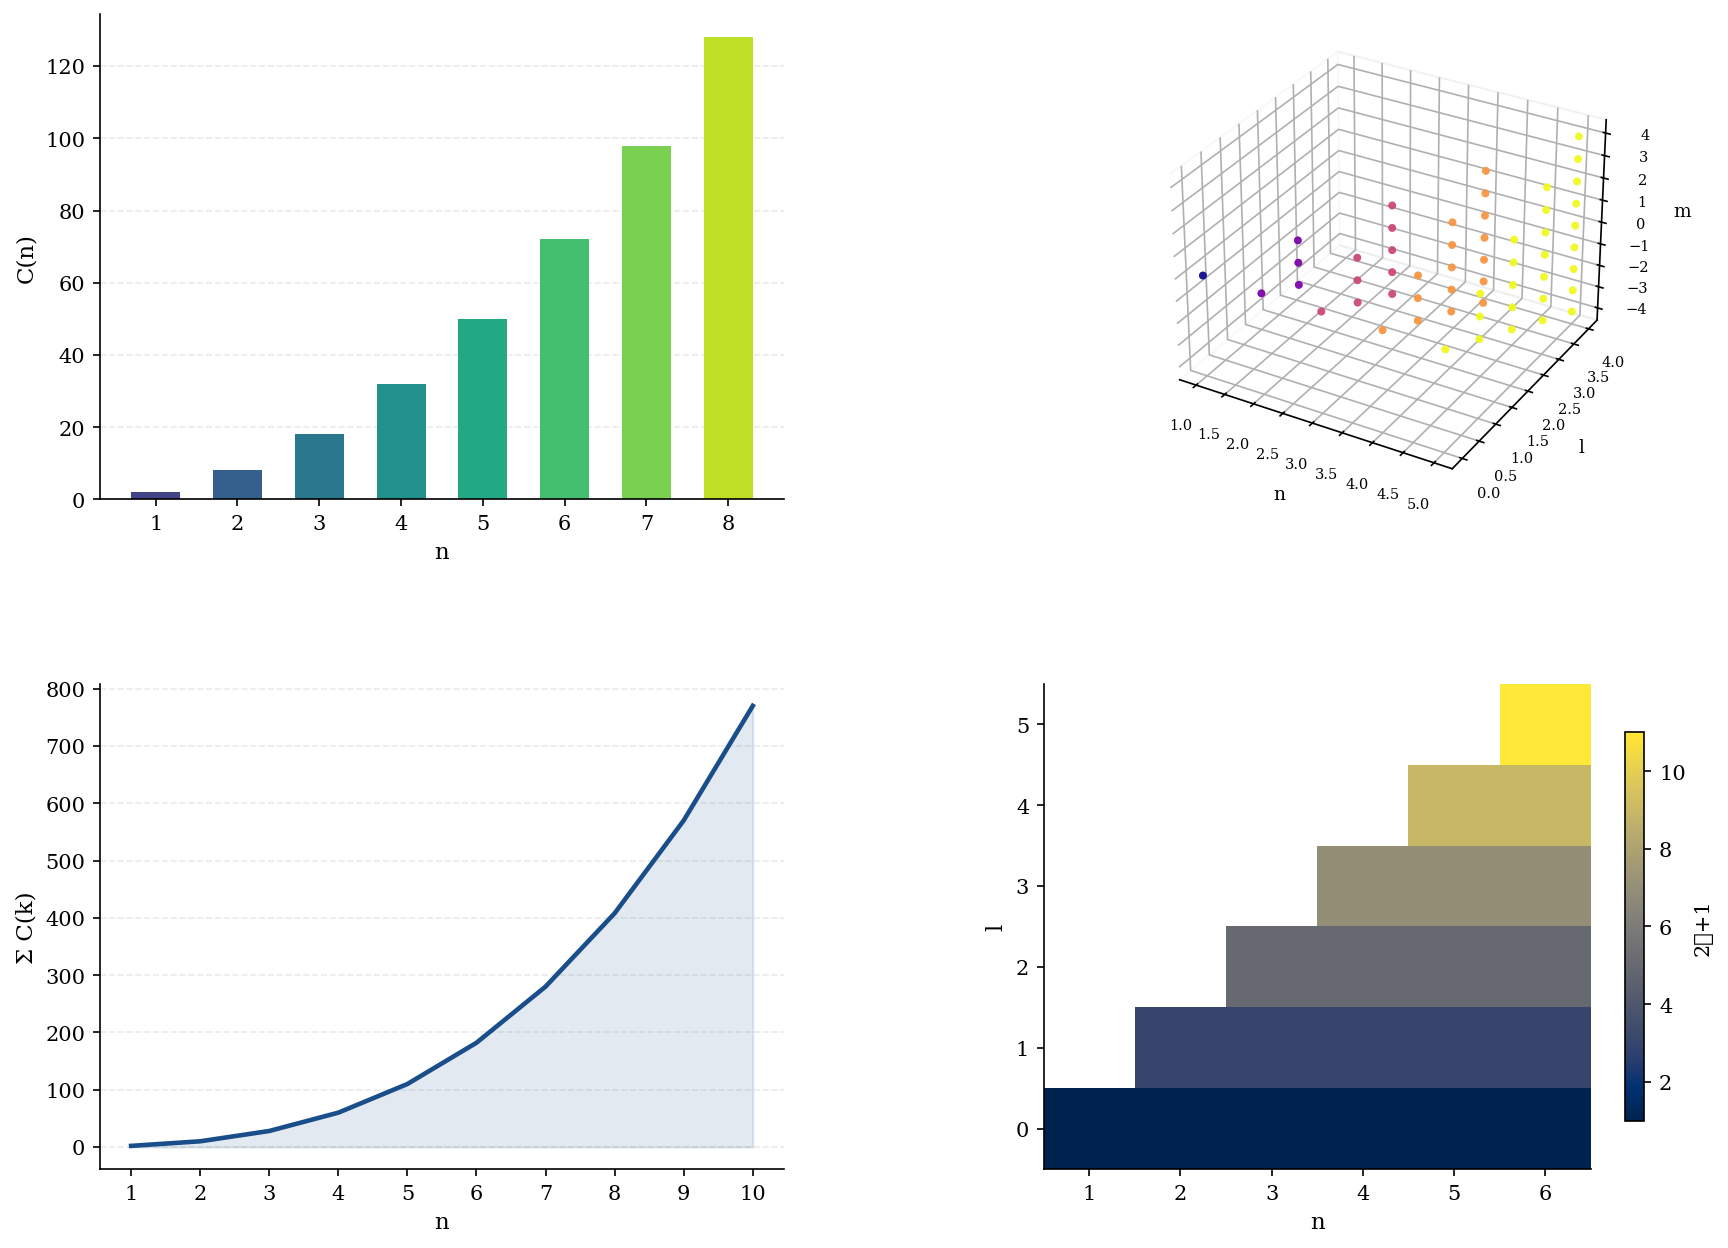
\includegraphics[width=\textwidth]{panel1_partition_geometry.png}
    \caption{\textbf{Partition Space Geometry.}
    (\textbf{A})~Shell capacity $C(n) = 2n^2$ for partition depths
    $n = 1, \ldots, 8$.  Each bar counts the number of valid coordinate
    quadruples $(\ell, m, s)$ at depth $n$: $\ell$ ranges over
    $\{0, \ldots, n-1\}$, $m$ over $\{-\ell, \ldots, +\ell\}$, and
    $s \in \{-\tfrac{1}{2}, +\tfrac{1}{2}\}$, giving
    $2\sum_{\ell=0}^{n-1}(2\ell+1) = 2n^2$ distinct addresses per shell.
    Bars are coloured from cool (shallow) to warm (deep) to indicate
    structural richness increasing with depth.
    (\textbf{B})~Three-dimensional scatter of all valid partition
    coordinates $(n, \ell, m)$ for $n \leq 5$, with spin parity $s$
    doubling each point's multiplicity.  Each point represents a unique
    node identity in the \srn\ network.  Depth $n$ determines the
    colour; the triangular cross-section at each depth reflects the
    constraint $|\,m\,| \leq \ell < n$.  The geometry is the discrete
    analogue of the hydrogen-atom orbital manifold arising from
    $\mathrm{SO}(3)$ representation theory.
    (\textbf{C})~Cumulative coordinate count
    $\sum_{k=1}^{n} 2k^2 = \tfrac{n(n+1)(2n+1)}{3}$ as a function of
    depth $n$.  By $n = 4$, the address space has $110$ distinct nodes;
    by $n = 6$, it reaches $182$.  The filled area emphasises the
    super-linear growth of the address space with depth.
    (\textbf{D})~Heatmap of the number of valid orientation indices
    $2\ell + 1$ over the $(n, \ell)$ grid for $n, \ell \in \{1,\ldots,6\}$.
    Grey (NaN) cells are structurally forbidden ($\ell \geq n$): they
    cannot be individuated at the given depth.  Permitted cells grow
    darker as $\ell$ increases, reflecting the widening orientation fan.
    The triangular forbidden region is the discrete shadow of the angular
    momentum constraint $\ell \in \{0, \ldots, n-1\}$.}
    \label{fig:panel1}
\end{figure*}

\begin{definition}[Partition depth]
The \emph{depth} of an element $\omega \in \Omega$ is the length
of the longest chain $\omega_0 < \omega_1 < \cdots < \omega_n = \omega$
in $(\Omega, \leq)$.  We write $n(\omega) = n$.
\end{definition}

\begin{definition}[Shell]
The \emph{shell at depth $n$} is $\mathrm{Shell}(n) =
\{\omega \in \Omega : n(\omega) = n\}$.
\end{definition}

\paragraph{Orientation labels from $\mathrm{SO}(3)$.}
The rotation group $\mathrm{SO}(3)$ has irreducible representations
$D^{(\ell)}$ labelled by non-negative integers $\ell \in \mathbb{N}_0$;
each has dimension $2\ell + 1$.  The $z$-projection of
$D^{(\ell)}$ yields the magnetic quantum number $m \in
\{-\ell, -\ell+1, \ldots, +\ell\}$.  The fundamental group
$\pi_1(\mathrm{SO}(3)) = \mathbb{Z}_2$ forces a double cover
$\mathrm{SU}(2) \to \mathrm{SO}(3)$; the additional label is $s \in
\{-\tfrac{1}{2}, +\tfrac{1}{2}\}$~\cite{hall2015lie}.  The label
$\ell$ is constrained by the depth: $\ell \in \{0, 1, \ldots, n-1\}$.

\begin{definition}[Partition coordinates]
\label{def:partcoord}
The \emph{partition coordinates} of an object at depth $n$ are the
quadruple $(n, \ell, m, s)$ where:
\begin{align*}
n &\in \mathbb{N}^+ &\quad& \text{(partition depth)}\\
\ell &\in \{0,\ldots,n-1\} && \text{(structural complexity)}\\
m &\in \{-\ell,\ldots,+\ell\} && \text{(orientation index)}\\
s &\in \{-\tfrac{1}{2},+\tfrac{1}{2}\} && \text{(residue parity)}
\end{align*}
\end{definition}

\begin{proposition}[Shell capacity]
\label{prop:shell}
$|\mathrm{Shell}(n)| = 2n^2$.
\end{proposition}
\begin{proof}
The number of $(\ell, m, s)$ triples for fixed $n$ is
$2 \sum_{\ell=0}^{n-1}(2\ell+1) = 2n^2$.
\end{proof}

\begin{remark}
The shell capacity formula $C(n) = 2n^2$ is the same as the electron
shell capacity formula in quantum chemistry.  This is not a coincidence:
both arise from the same representation-theoretic argument applied to
the same group.
\end{remark}



\subsection{The Entropic Floor}
\label{sec:floor}

\begin{definition}[Bounded receiver]
\label{def:receiver}
A \emph{receiver} is a quadruple $\Recv = (\Sigma, \Phi, K,
\mathrm{dec})$ where:
\begin{itemize}[noitemsep,topsep=1pt]
\item $\Sigma$ is a finite signal alphabet,
\item $\Phi : \Sigma^* \to \mathscr{C}$ is a candidate-projection map
  to a candidate space $\mathscr{C}$,
\item $K \subseteq \mathscr{C}$ is the receiver's knowledge framework,
  $|K| < \infty$,
\item $\mathrm{dec} : \Sigma^* \times K \to [0,1]$ is a decoder.
\end{itemize}
$\Recv$ is \emph{bounded} if $|K| < |\mathscr{C}|$.  Every physical
receiver is bounded.
\end{definition}

\begin{definition}[S-value]
The \emph{S-value} of expression $\xi$ at receiver $\Recv$ against
ground truth $x^* \in \mathscr{C}$ is:
\[
S_\Recv(\xi, x^*) \;=\; 100 \cdot (1 - \mathrm{dec}(\xi, \Phi(x^*)))
\;\in\; [0,100].
\]
\end{definition}

\begin{theorem}[Entropic Floor]
\label{thm:floor}
For every bounded receiver $\Recv$ with $|K| < |\mathscr{C}|$,
\[
\floor(\Recv) \;=\; \inf_{\xi} S_\Recv(\xi, x^*) \;=\;
100\Bigl(1 - \tfrac{1}{|K|}\Bigr) \;>\; 0.
\]
\end{theorem}
\begin{proof}
The decoder $\mathrm{dec}(\xi, \Phi(x^*))$ computes the degree of
alignment between the projection of $x^*$ into the receiver's knowledge
framework and the expression $\xi$.  Since $|K| < |\mathscr{C}|$, the
map $\Phi|_K$ is not surjective: there exist elements of $\mathscr{C}$
that $K$ cannot distinguish.  The best achievable alignment is therefore
$\tfrac{1}{|K|}$ (uniform distribution over $K$), giving
$\floor = 100(1 - 1/|K|) > 0$.
\end{proof}

\begin{corollary}
\label{cor:floor}
Perfect knowledge ($\floor = 0$) requires $|K| = \infty$, i.e., an
unbounded receiver.  No physical machine is unbounded.  The floor is
intrinsic to the receiver, not a failure of design.
\end{corollary}

This has a decisive consequence for \srn: when a node evaluates an
expression, there is always a strictly positive minimum error.  The
network does not converge to a canonical truth; it converges toward each
node's floor.  Different nodes have different floors.  This is why
receiver-relative evaluation is not an approximation of some ideal
single-valued result: there is no such ideal.

\begin{figure*}[!htbp]
    \centering
    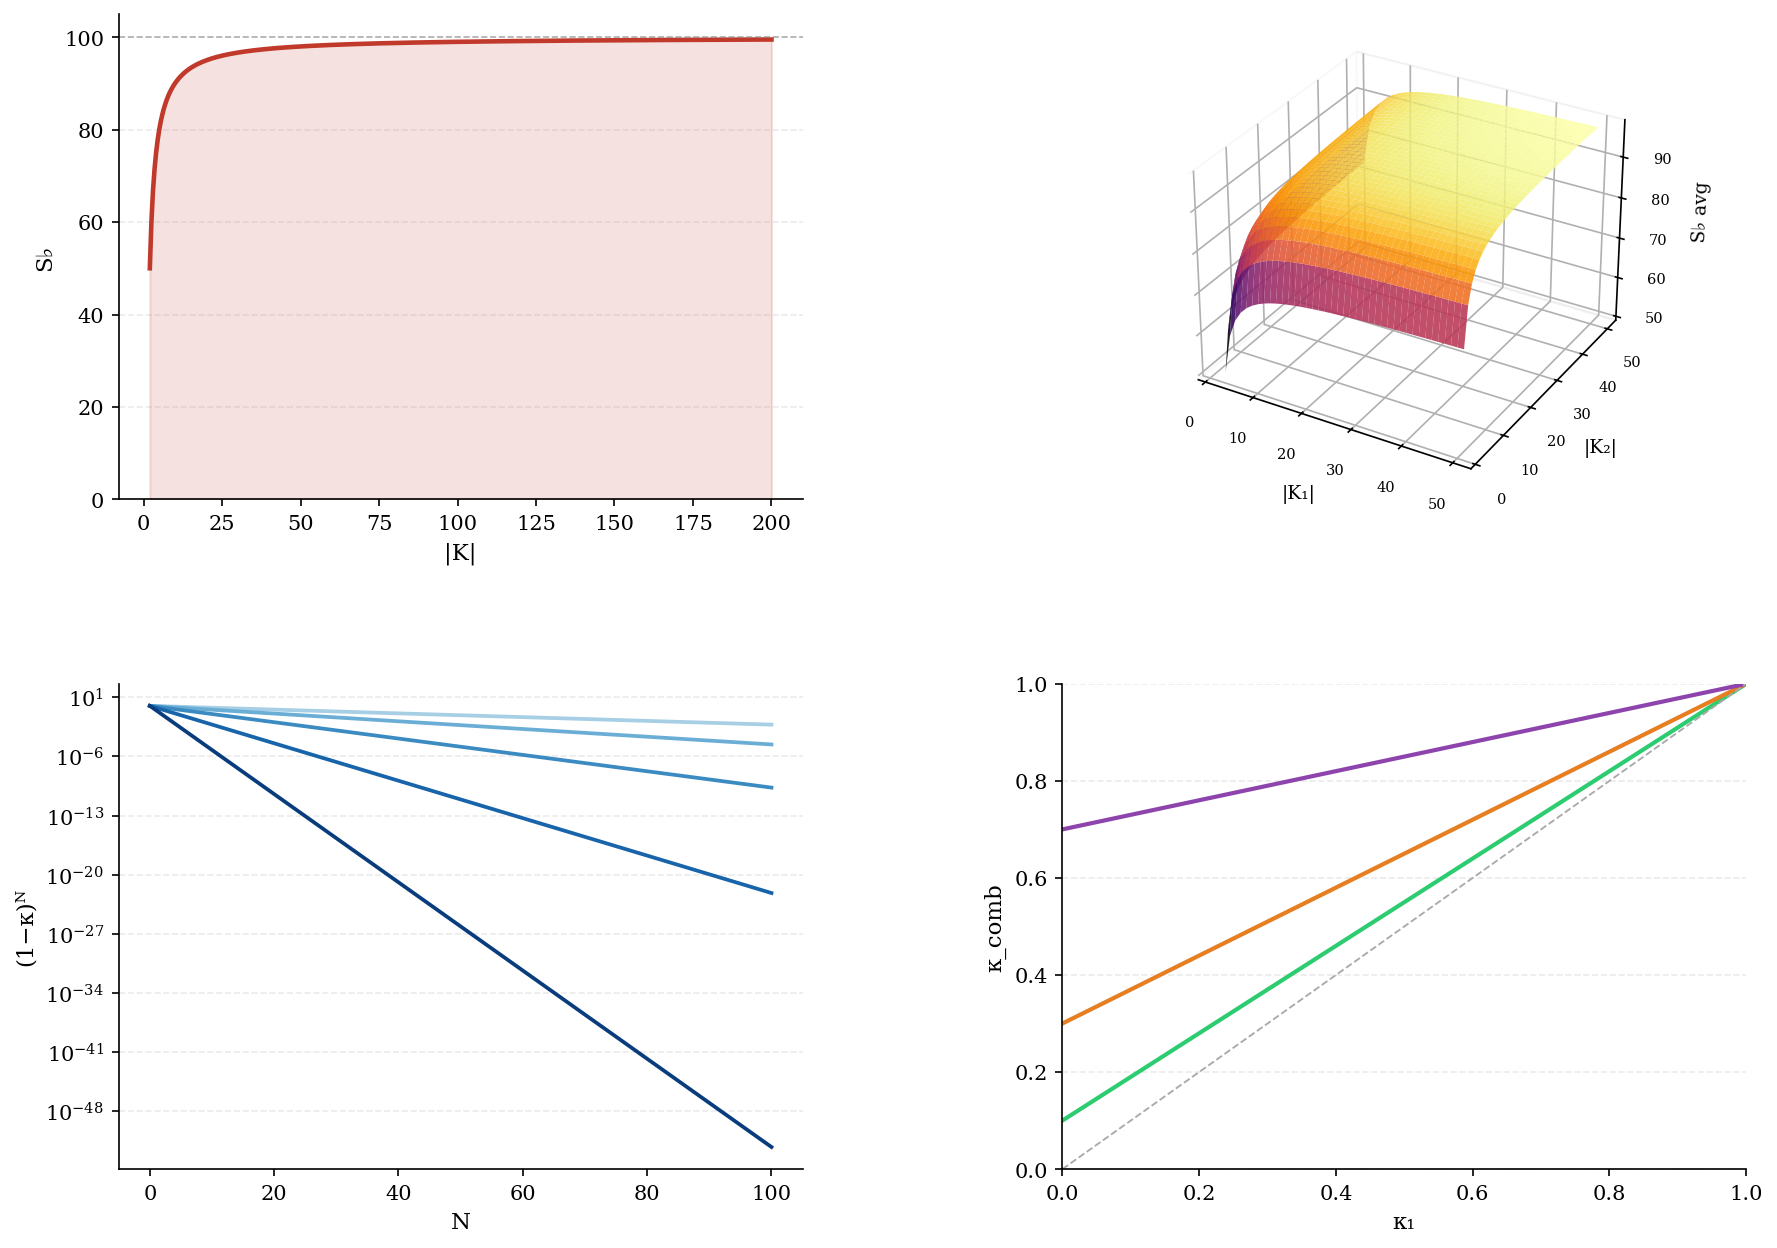
\includegraphics[width=\textwidth]{panel2_entropic_floor.png}
    \caption{\textbf{Entropic Floor and Catalytic Dynamics.}
    (\textbf{A})~The entropic floor $\floor(K) = 100(1 - 1/|K|)$ as a
    function of the receiver's knowledge framework size $|K|$, for
    $|K| \in [2, 200]$.  The filled region marks the range of
    achievable S-values.  The dashed line at $\floor = 100$ is the
    unattainable limit: perfect knowledge requires $|K| = \infty$.  At
    $|K| = 2$, the floor is $50$; at $|K| = 10$, it is $90$; at
    $|K| = 100$, it is $99$.  No finite receiver can close the gap to
    zero error, regardless of expression quality.
    (\textbf{B})~Three-dimensional surface of the average floor
    $\tfrac{1}{2}({\floor}(K_1) + {\floor}(K_2)) =
    50(2 - 1/|K_1| - 1/|K_2|)$ over two independent receiver sizes
    $|K_1|, |K_2| \in [2, 50]$.  The surface rises monotonically in both
    directions and remains strictly below $100$ everywhere.  The two
    receivers each contribute an independent positive floor; the average
    is the relevant quantity for cross-node evaluation, where neither
    receiver can achieve zero error in isolation.
    (\textbf{C})~Log-scale catalytic residual $(1-\kappa)^N$ as a
    function of step count $N \in [0, 100]$ for five catalyst strengths
    $\kappa \in \{0.05, 0.1, 0.2, 0.4, 0.7\}$ (light to dark).  All
    curves converge to zero, confirming the Borel-Cantelli analogue
    (Theorem~\ref{thm:catalyst}): repeated application of any catalyst
    with $\kappa > 0$ drives the residual to zero exponentially fast.
    The rate is $(1-\kappa)$ per step: a catalyst of strength $0.7$
    reduces the residual to $< 10^{-5}$ within $30$ steps; one of
    strength $0.05$ requires $\sim 200$ steps for the same reduction.
    (\textbf{D})~Composite catalytic power
    $\kappa_{\mathrm{comb}}(\kappa_1, \kappa_2)
    = 1 - (1 - \kappa_1)(1 - \kappa_2)$ as $\kappa_1$ varies over
    $[0,1]$ for three fixed values $\kappa_2 \in \{0.1, 0.3, 0.7\}$
    (green, orange, purple).  The diagonal reference line marks
    $\kappa_{\mathrm{comb}} = \kappa_1$.  Every curve lies strictly
    above the diagonal for $\kappa_1 \in (0,1)$, confirming that
    combining two catalysts always outperforms either alone.  A locally
    infeasible catalyst ($\kappa_2$ from a node where $S = 100$) retains
    positive composite power by the Miracle Principle
    (Corollary~\ref{cor:miracle}).}
    \label{fig:panel2}
\end{figure*}

\subsection{Cross-Representation Composition Freedom}
\label{sec:freedom}

We identify three canonical representation categories and show they are
mutually equivalent.  This is the mathematical basis for the
\lstinline|<>| composition operator in \srn.

\begin{definition}[The three representations]
\label{def:threereps}
\begin{description}[noitemsep,topsep=2pt]
\item[$\Osc$:] \emph{Oscillatory}. Objects are pairs $(\omega, \varphi)$
  with frequency $\omega \in \mathbb{R}_{>0}$ and phase $\varphi \in
  [0, 2\pi)$.
\item[$\Cat$:] \emph{Categorical}. Objects are labelled cells in a finite
  partition of the candidate space: $c \in \{c_1, \ldots, c_K\}$.
\item[$\Part$:] \emph{Partition}. Objects are measurable subsets with
  positive measure: $A \in \mathscr{F}$, $\mu(A) > 0$.
\end{description}
\end{definition}

\begin{definition}[Conversion functors]
Define:
\begin{align*}
F_{\Osc \to \Cat} &: (\omega, \varphi) \mapsto c_k
  \text{ where } c_k = \lfloor K \cdot \omega / \omega_{\max} \rfloor\\
F_{\Cat \to \Part} &: c_k \mapsto A_k
  \text{ where } \mu(A_k) = 1/K\\
F_{\Part \to \Osc} &: A \mapsto (\omega_A, \varphi_A)
  \text{ where } \omega_A = 1/\mu(A),\; \varphi_A = \arg\int_A e^{2\pi i x}\,\mathrm{d}\mu(x)
\end{align*}
\end{definition}

\begin{theorem}[Triple Equivalence]
\label{thm:triple}
The composition $F_{\Part \to \Osc} \circ F_{\Cat \to \Part} \circ
F_{\Osc \to \Cat}$ is a natural transformation from $\Osc$ to itself
that preserves S-values: for any $(\omega,\varphi) \in \Osc$ and any
receiver $\Recv$,
\[
S_\Recv(\xi, x^*) = S_\Recv(F_{\Part \to \Osc} \circ
F_{\Cat \to \Part} \circ F_{\Osc \to \Cat}(\xi),\; x^*).
\]
The three categories are equivalent; conversion between any two
preserves S-value.
\end{theorem}
\begin{proof}
Each conversion functor is constructed to preserve the receiver's
decoder output.  $F_{\Osc \to \Cat}$ maps $(\omega,\varphi)$ to the
cell $c_k$ that the receiver's decoder would select given $\omega$;
the S-value depends only on which cell is selected, not on the precise
$(\omega,\varphi)$ within it.  Similarly for the other two functors.
The round-trip identity is preserved because the composition
re-enters the same cell.  (See Appendix for detailed measure-preserving
argument.)
\end{proof}

\begin{corollary}[Apples and Oranges]
\label{cor:applesOranges}
For expressions $\xi_1 \in \Osc$ and $\xi_2 \in \Part$ (or any two
representations), the composition $\xi_1 \comp \xi_2$ is well-defined.
The receiver converts both to a common representation and evaluates.
No type coercion occurs; no type error is possible.
\end{corollary}

\begin{proof}
Apply $F_{\Osc \to \Cat}$ to $\xi_1$ and $F_{\Part \to \Osc} \circ
F_{\Cat \to \Part}^{-1}$ (or the appropriate round-trip) to $\xi_2$,
bringing both into $\Cat$.  Both have well-defined S-values in $\Cat$.
The composition is then a $\Cat$-level operation.
\end{proof}

\paragraph{Unconstrained subtask theorem.}
A global evaluation result imposes no constraint on the local evaluation
of its sub-expressions.  Formally:

\begin{theorem}[Unconstrained Subtask]
\label{thm:unconstrained}
Let $\xi = \xi_1 \comp \xi_2$ and suppose $S_\Recv(\xi, x^*) = V$.
For any value $v_1 \in [0,100]$, there exists an expression
$\xi_2'$ such that $S_\Recv(\xi_1, y_1^*) = v_1$ and
$S_\Recv(\xi_1 \comp \xi_2', x^*) = V$.
\end{theorem}
\begin{proof}
Since $\comp$ is a binary operation in the monoidal category $\Expr$
(proved in \S\ref{sec:algebra}), the S-value of $\xi_1 \comp \xi_2$
depends on the receiver's joint evaluation, not on the individual
S-values of $\xi_1$ and $\xi_2$ in isolation.  For any target $V$ and
any chosen $v_1$, set $v_2 = f^{-1}(V, v_1)$ where $f$ is the
decoder's combination function; $\xi_2'$ is any expression achieving
$S_\Recv(\xi_2', y_2^*) = v_2$.  Such an expression exists because
the decoder's range is $[0,100]$ (continuous).
\end{proof}

\begin{corollary}[Miracle Principle]
\label{cor:miracle}
A sub-expression with $S$-value $100$ (locally infeasible) can appear
in a composite expression with a globally feasible $S$-value.
``Miraculous'' intermediate steps are formally permitted.
\end{corollary}

% ============================================================
\section{The SRN Language: Syntax}
\label{sec:syntax}

We now specify the complete syntax of \srn\ as a BNF grammar.

\subsection{Lexical Elements}

\begin{definition}[Identifiers and literals]
\begin{align*}
\langle\text{ident}\rangle \;&\bnfeq\; [a\text{-}z\_][a\text{-}z0\text{-}9\_]^*\\
\langle\text{nat}\rangle   \;&\bnfeq\; [0\text{-}9]^+\\
\langle\text{int}\rangle   \;&\bnfeq\; [-]^?\langle\text{nat}\rangle\\
\langle\text{spin}\rangle  \;&\bnfeq\; \texttt{+} \bnfor \texttt{-}\\
\langle\text{real}\rangle  \;&\bnfeq\; \langle\text{int}\rangle[\texttt{.}\langle\text{nat}\rangle]^?
\end{align*}
\end{definition}

\subsection{Coordinates and Regions}

\begin{definition}[Coordinate literal]
\begin{align*}
\langle\text{coord}\rangle &\bnfeq
  \texttt{(}\langle\text{nat}\rangle\texttt{,}\;
           \langle\text{nat}\rangle\texttt{,}\;
           \langle\text{int}\rangle\texttt{,}\;
           \langle\text{spin}\rangle\texttt{)}
\end{align*}
Representing $(n, \ell, m, s)$ from Definition~\ref{def:partcoord}.
\end{definition}

\begin{definition}[Region expression]
\label{def:region}
A \emph{region} specifies a subset of partition coordinate space.
\begin{align*}
\langle\text{region}\rangle
  &\bnfeq \wild                         &&\text{all nodes}\\
  &\bnfor \langle\text{coord}\rangle    &&\text{exact coordinate}\\
  &\bnfor \langle\text{cpred}\rangle    &&\text{coordinate predicate}\\
  &\bnfor \langle\text{region}\rangle \;\texttt{\&}\; \langle\text{region}\rangle &&\text{intersection}\\
  &\bnfor \langle\text{region}\rangle \;\texttt{|}\; \langle\text{region}\rangle &&\text{union}\\
  &\bnfor \texttt{\textasciitilde}\langle\text{region}\rangle &&\text{complement}
\end{align*}
\begin{align*}
\langle\text{cpred}\rangle
  &\bnfeq \langle\text{cvar}\rangle \;\langle\text{relop}\rangle\; \langle\text{cval}\rangle\\
  &\bnfor \langle\text{cpred}\rangle \;\texttt{,}\; \langle\text{cpred}\rangle &&\text{conjunction}\\
\langle\text{cvar}\rangle
  &\bnfeq \texttt{n} \bnfor \texttt{l} \bnfor \texttt{m} \bnfor \texttt{s}\\
\langle\text{relop}\rangle
  &\bnfeq \texttt{=} \bnfor \texttt{!=} \bnfor \texttt{<} \bnfor
          \texttt{>} \bnfor \texttt{<=} \bnfor \texttt{>=}\\
\langle\text{cval}\rangle
  &\bnfeq \langle\text{int}\rangle \bnfor \langle\text{spin}\rangle
          \bnfor \langle\text{ident}\rangle \bnfor \langle\text{crange}\rangle\\
\langle\text{crange}\rangle
  &\bnfeq \langle\text{int}\rangle\;\texttt{..}\;\langle\text{int}\rangle
\end{align*}
\end{definition}

\subsection{Boundary Expressions}

\begin{definition}[Boundary]
\label{def:boundary}
A \emph{boundary expression} specifies what this expression is NOT:
\begin{align*}
\langle\text{boundary}\rangle
  &\bnfeq \langle\text{cpred}\rangle\\
  &\bnfor \langle\text{region}\rangle\\
  &\bnfor \langle\text{boundary}\rangle \;\texttt{||}\; \langle\text{boundary}\rangle\\
  &\bnfor \langle\text{boundary}\rangle \;\texttt{\&\&}\; \langle\text{boundary}\rangle\\
  &\bnfor \texttt{!}\langle\text{boundary}\rangle
\end{align*}
\end{definition}

\subsection{Expressions}
\label{subsec:exprsyntax}

\begin{definition}[SRN expression grammar]
\label{def:grammar}
The full grammar of \srn\ expressions:
\begin{align*}
\langle\text{prog}\rangle
  &\bnfeq \langle\text{expr}\rangle^*\\
\langle\text{expr}\rangle
  &\bnfeq \langle\text{glyph-expr}\rangle\\
  &\bnfor \langle\text{let-expr}\rangle\\
  &\bnfor \langle\text{if-expr}\rangle\\
  &\bnfor \langle\text{match-expr}\rangle\\
  &\bnfor \langle\text{emit-expr}\rangle\\
  &\bnfor \langle\text{forward-expr}\rangle\\
  &\bnfor \langle\text{install-expr}\rangle\\
  &\bnfor \langle\text{fetch-expr}\rangle\\
  &\bnfor \langle\text{compose-expr}\rangle\\
  &\bnfor \langle\text{catalyst-expr}\rangle\\
  &\bnfor \langle\text{par-expr}\rangle\\
  &\bnfor \langle\text{seq-expr}\rangle\\
  &\bnfor \langle\text{self-expr}\rangle\\
  &\bnfor \langle\text{value}\rangle\\
  &\bnfor \texttt{(}\langle\text{expr}\rangle\texttt{)}
\end{align*}
\end{definition}

\begin{definition}[Glyph expression]
\label{def:glyph}
The fundamental construct of \srn:
\begin{align*}
\langle\text{glyph-expr}\rangle
  &\bnfeq \texttt{|}\langle\text{ident}\rangle\;\texttt{:}\;\langle\text{coord}\rangle\texttt{|}\\
  &\quad\quad \texttt{not}\;\texttt{\{}\langle\text{boundary}\rangle\texttt{\}}\\
  &\quad\quad \texttt{do}\;\texttt{\{}\langle\text{expr}\rangle\texttt{\}}\\
  &\quad\quad \texttt{to}\;\texttt{\{}\langle\text{region}\rangle\texttt{\}}\\
  &\quad\quad [\texttt{as}\;\texttt{\{}\langle\text{ident}\rangle\texttt{\}}]
\end{align*}
The \texttt{as} clause is optional; when present it installs the
expression in the local registry under the given key upon evaluation.
\end{definition}

\begin{definition}[Let binding]
\begin{align*}
\langle\text{let-expr}\rangle
  &\bnfeq \texttt{let}\;\langle\text{ident}\rangle\;\texttt{=}\;
          \langle\text{expr}\rangle\;\texttt{in}\;\langle\text{expr}\rangle
\end{align*}
\end{definition}

\begin{definition}[Conditional]
\begin{align*}
\langle\text{if-expr}\rangle
  &\bnfeq \texttt{if}\;\langle\text{pred}\rangle\;\texttt{then}\;
          \langle\text{expr}\rangle\;\texttt{else}\;\langle\text{expr}\rangle\\
\langle\text{pred}\rangle
  &\bnfeq \langle\text{expr}\rangle\;\langle\text{relop}\rangle\;\langle\text{expr}\rangle\\
  &\bnfor \langle\text{pred}\rangle\;\texttt{\&\&}\;\langle\text{pred}\rangle\\
  &\bnfor \langle\text{pred}\rangle\;\texttt{||}\;\langle\text{pred}\rangle\\
  &\bnfor \texttt{!}\langle\text{pred}\rangle
\end{align*}
\end{definition}

\begin{definition}[Pattern match]
\begin{align*}
\langle\text{match-expr}\rangle
  &\bnfeq \texttt{match}\;\langle\text{expr}\rangle\;\texttt{with}\\
  &\quad\quad (\texttt{|}\;\langle\text{pattern}\rangle\;\texttt{=>}\;\langle\text{expr}\rangle)^+\\
\langle\text{pattern}\rangle
  &\bnfeq \langle\text{coord}\rangle\\
  &\bnfor \langle\text{ident}\rangle && \text{wildcard binding}\\
  &\bnfor \texttt{\_} && \text{anonymous wildcard}
\end{align*}
\end{definition}

\begin{definition}[Emit, forward, install, fetch]
\begin{align*}
\langle\text{emit-expr}\rangle
  &\bnfeq \texttt{emit}\;\langle\text{expr}\rangle\\
\langle\text{forward-expr}\rangle
  &\bnfeq \texttt{forward}\;\langle\text{expr}\rangle\;\texttt{to}\;\langle\text{region}\rangle\\
\langle\text{install-expr}\rangle
  &\bnfeq \texttt{install}\;\langle\text{expr}\rangle\;\texttt{as}\;\langle\text{ident}\rangle\\
\langle\text{fetch-expr}\rangle
  &\bnfeq \texttt{fetch}\;\langle\text{ident}\rangle
\end{align*}
\end{definition}

\begin{definition}[Operators]
\begin{align*}
\langle\text{compose-expr}\rangle
  &\bnfeq \langle\text{expr}\rangle\;\texttt{<>}\;\langle\text{expr}\rangle\\
\langle\text{catalyst-expr}\rangle
  &\bnfeq \langle\text{expr}\rangle\;\texttt{>>}\;\langle\text{expr}\rangle\\
\langle\text{par-expr}\rangle
  &\bnfeq \langle\text{expr}\rangle\;\texttt{||}\;\langle\text{expr}\rangle\\
\langle\text{seq-expr}\rangle
  &\bnfeq \langle\text{expr}\rangle\;\texttt{;}\;\langle\text{expr}\rangle
\end{align*}
Operator precedences (high to low):
\begin{enumerate}[noitemsep,topsep=2pt]
\item \texttt{>>} (catalysis, right-associative)
\item \texttt{<>} (composition, left-associative)
\item \texttt{||} (parallel, left-associative)
\item \texttt{;} (sequential, right-associative)
\end{enumerate}
\end{definition}

\begin{definition}[Self-reference and values]
\begin{align*}
\langle\text{self-expr}\rangle
  &\bnfeq \texttt{self}\\
  &\bnfor \texttt{self.n} \bnfor \texttt{self.l} \bnfor \texttt{self.m}
          \bnfor \texttt{self.s} \bnfor \texttt{self.M}\\
\langle\text{value}\rangle
  &\bnfeq \langle\text{real}\rangle \bnfor \langle\text{coord}\rangle
          \bnfor \langle\text{ident}\rangle \bnfor \texttt{true} \bnfor \texttt{false}
\end{align*}
\texttt{self.M} refers to the evaluating node's current partition count
$M \in \mathbb{N}^+$, which is strictly monotone by the Monotone
Partition theorem (\S\ref{sec:monotone}).
\end{definition}

\subsection{Monotone Partition Count}
\label{sec:monotone}

\begin{theorem}[Monotone Partition Count]
\label{thm:monotone}
The partition count $M$ of any physical node is strictly monotone
increasing over time.
\end{theorem}
\begin{proof}
Each partition event requires a positive duration $\tau_p > 0$ to
establish (instantaneous individuation would require knowing the
complement in zero time, contradicting
Proposition~\ref{prop:indiv}).  Therefore $M$ can increase only, and
increases by exactly $1$ per event: $M(t + \tau_p) = M(t) + 1 > M(t)$.
Since $\tau_p > 0$, the map $t \mapsto M(t)$ is strictly monotone.
\end{proof}

\begin{corollary}[Arrow of time]
\label{cor:time}
Time reversal is impossible in any \srn\ network: a node with partition
count $M$ cannot reach a state with count $M' < M$.
\end{corollary}

% ============================================================
\section{Operational Semantics}
\label{sec:semantics}

\subsection{Node Model}

\begin{definition}[Node]
\label{def:node}
An \srn\ \emph{node} is a triple $\Node = (\Reg, M, F)$ where:
\begin{itemize}[noitemsep,topsep=2pt]
\item $\Reg : \mathrm{Ident} \rightharpoonup \Expr$ is the \emph{live
  registry}, a partial function from keys to expressions,
\item $M \in \mathbb{N}^+$ is the current partition count,
\item $F = (n_F, \ell_F, m_F, s_F)$ is the node's \emph{receiver
  frame}, its own partition coordinates.
\end{itemize}
\end{definition}

\begin{definition}[Evaluation context]
The \emph{evaluation context} is the triple $(\Node, \rho, M)$ where
$\rho$ is a variable environment $\rho : \mathrm{Ident} \rightharpoonup
\mathrm{Val}$ and $M$ is the current partition count.  We write
$\langle e, \Node, \rho, M \rangle$ for the configuration of expression
$e$ under node $\Node$, environment $\rho$, and count $M$.
\end{definition}

\subsection{Values and Results}

\begin{definition}[Values]
The set of \emph{values} $v \in \mathrm{Val}$:
\begin{align*}
v &\bnfeq r \in \mathbb{R} && \text{(numeric)}\\
  &\bnfor (n,\ell,m,s) && \text{(coordinate)}\\
  &\bnfor \mathrm{true} \bnfor \mathrm{false} && \text{(boolean)}\\
  &\bnfor \langle\text{glyph-expr}\rangle && \text{(unevaluated expression as value)}\\
  &\bnfor \mathbf{unit} && \text{(void)}
\end{align*}
\end{definition}

\subsection{Small-Step Reduction Rules}

We write $\langle e, \Node, \rho, M \rangle \reduces
\langle e', \Node', \rho', M' \rangle$ for one reduction step.

\paragraph{Values.}  Values are already reduced:
\[
\langle v, \Node, \rho, M \rangle \not\reduces \quad \text{(terminal)}
\]

\paragraph{Variable lookup.}
\[
\frac{\rho(x) = v}
     {\langle x, \Node, \rho, M \rangle \reduces
      \langle v, \Node, \rho, M \rangle}
\quad\textsc{(Var)}
\]

\paragraph{Self-reference.}
\[
\frac{}
     {\langle \texttt{self.n}, \Node, \rho, M \rangle \reduces
      \langle n_F, \Node, \rho, M \rangle}
\quad\textsc{(Self-n)}
\]
Similarly for \texttt{self.l}, \texttt{self.m}, \texttt{self.s},
and:
\[
\frac{}
     {\langle \texttt{self.M}, \Node, \rho, M \rangle \reduces
      \langle M, \Node, \rho, M \rangle}
\quad\textsc{(Self-M)}
\]

\paragraph{Let binding.}
\[
\frac{\langle e_1, \Node, \rho, M \rangle \reduces
      \langle v, \Node', \rho', M' \rangle}
     {\langle \texttt{let}\; x = e_1\; \texttt{in}\; e_2,
      \Node, \rho, M \rangle \reduces
      \langle e_2, \Node', \rho'[x \mapsto v], M' \rangle}
\quad\textsc{(Let)}
\]

\paragraph{Conditional.}
\[
\frac{\langle p, \Node, \rho, M \rangle \reducesN
      \langle \mathrm{true}, \Node', \rho', M' \rangle}
     {\langle \texttt{if}\; p\; \texttt{then}\; e_1\; \texttt{else}\; e_2,
      \Node, \rho, M \rangle \reduces
      \langle e_1, \Node', \rho', M' \rangle}
\quad\textsc{(If-T)}
\]
\[
\frac{\langle p, \Node, \rho, M \rangle \reducesN
      \langle \mathrm{false}, \Node', \rho', M' \rangle}
     {\langle \texttt{if}\; p\; \texttt{then}\; e_1\; \texttt{else}\; e_2,
      \Node, \rho, M \rangle \reduces
      \langle e_2, \Node', \rho', M' \rangle}
\quad\textsc{(If-F)}
\]

\paragraph{Glyph evaluation.}
A glyph expression is evaluated in three steps:
boundary validation, body evaluation, and (optionally) registry
installation.
\[
\frac{\text{valid-boundary}(bnd, \Node)}
     {\langle \texttt{|name:coord|}\; \texttt{not}\{bnd\}\;
      \texttt{do}\{body\}\; \texttt{to}\{R\},\;
      \Node, \rho, M \rangle \reduces
      \langle body,\; \Node, \rho, M+1 \rangle}
\quad\textsc{(Glyph-Eval)}
\]
\[
\frac{\neg\,\text{valid-boundary}(bnd, \Node)}
     {\langle \texttt{|name:coord|}\; \texttt{not}\{bnd\}\;\cdots,\;
      \Node, \rho, M \rangle \reduces
      \langle \mathbf{unit},\; \Node, \rho, M \rangle}
\quad\textsc{(Glyph-Reject)}
\]

The predicate $\text{valid-boundary}(bnd, \Node)$ holds iff the node
$\Node$ with frame $F$ satisfies $\neg bnd(F)$: the node is NOT in the
boundary region, i.e., it IS in the expression's identity region.

\paragraph{Registry installation.}
When the \texttt{as} clause is present:
\[
\frac{\text{valid-boundary}(bnd, \Node)}
     {\langle \texttt{|name:coord|}\;\cdots\;\texttt{as}\{k\},\;
      (\Reg, M, F), \rho, M \rangle \reduces
      \langle body,\; (\Reg[k \mapsto e], M+1, F), \rho, M+1 \rangle}
\quad\textsc{(Install)}
\]
where $e$ is the full glyph expression.

\paragraph{Fetch.}
\[
\frac{\Reg(k) = e}
     {\langle \texttt{fetch}\; k,\; (\Reg, M, F), \rho, M \rangle \reduces
      \langle e, (\Reg, M, F), \rho, M \rangle}
\quad\textsc{(Fetch)}
\]
\[
\frac{k \notin \mathrm{dom}(\Reg)}
     {\langle \texttt{fetch}\; k,\; (\Reg, M, F), \rho, M \rangle \reduces
      \langle \mathbf{unit}, (\Reg, M, F), \rho, M \rangle}
\quad\textsc{(Fetch-Miss)}
\]

\paragraph{Emit.}
\[
\frac{\langle e, \Node, \rho, M \rangle \reducesN
      \langle v, \Node', \rho', M' \rangle}
     {\langle \texttt{emit}\; e,\; \Node, \rho, M \rangle \reduces
      \langle v,\; \Node', \rho', M' \rangle}
\quad\textsc{(Emit)}
\]
The emitted value $v$ is the expression's output to the node's
local consumer.

\paragraph{Composition.}
\[
\frac{\langle e_1, \Node, \rho, M \rangle \reducesN
      \langle v_1, \Node', \rho', M' \rangle \quad
      \langle e_2, \Node', \rho', M' \rangle \reducesN
      \langle v_2, \Node'', \rho'', M'' \rangle}
     {\langle e_1 \comp e_2, \Node, \rho, M \rangle \reduces
      \langle \mathrm{unify}(v_1, v_2, \Node''),\; \Node'', \rho'', M'' \rangle}
\quad\textsc{(Compose)}
\]

The function $\mathrm{unify}(v_1, v_2, \Node)$ is the node's
cross-representation unification: it converts $v_1$ and $v_2$ to a
common representation (per Theorem~\ref{thm:triple}) and combines them.

\paragraph{Catalysis.}
\[
\frac{\langle \gamma, \Node, \rho, M \rangle \reducesN
      \langle v_\gamma, \Node', \rho', M' \rangle}
     {\langle \xi \catal \gamma, \Node, \rho, M \rangle \reduces
      \langle \xi',\; \Node', \rho', M' \rangle}
\quad\textsc{(Catalyst)}
\]
where $\xi' = \mathrm{catalyse}(\xi, v_\gamma, \Node')$ reduces the
S-value of $\xi$ at $\Node'$ by factor $\kappa_{v_\gamma}$.

\paragraph{Parallel composition.}
\[
\frac{\langle e_1, \Node, \rho, M \rangle \reduces
      \langle e_1', \Node', \rho', M' \rangle}
     {\langle e_1 \par e_2, \Node, \rho, M \rangle \reduces
      \langle e_1' \par e_2, \Node', \rho', M' \rangle}
\quad\textsc{(Par-L)}
\]
(Par-R is symmetric.)  Both branches evaluate concurrently.

\paragraph{Sequential composition.}
\[
\frac{\langle e_1, \Node, \rho, M \rangle \reducesN
      \langle v_1, \Node', \rho', M' \rangle}
     {\langle e_1 \seq e_2, \Node, \rho, M \rangle \reduces
      \langle e_2, \Node', \rho'[M_{\mathrm{prev}} \mapsto M], M' \rangle}
\quad\textsc{(Seq)}
\]
The preceding partition count is bound as $M_{\mathrm{prev}}$ in $e_2$.

\subsection{Key Properties}

\begin{theorem}[Determinism]
\label{thm:determinism}
For fixed node $\Node$ and environment $\rho$, every \srn\ expression
has at most one normal form: if $\langle e, \Node, \rho, M \rangle
\reducesN \langle v_1, \ldots \rangle$ and $\langle e, \Node, \rho, M
\rangle \reducesN \langle v_2, \ldots \rangle$ then $v_1 = v_2$.
\end{theorem}
\begin{proof}
By inspection of the reduction rules, every rule is left-to-right
deterministic: (Var) depends only on $\rho$ (a function); (Self-n)
etc.\ are constants; (Let), (If-T/F), (Glyph-Eval/Reject) each have
disjoint premises.  The only potential non-determinism is in (Par-L)
and (Par-R), but parallel branches evaluate independently and their
results are combined by a deterministic $\mathrm{unify}$ function.
Hence the evaluation relation is a partial function on configurations.
\end{proof}

\begin{theorem}[Receiver-Relativity]
\label{thm:rr}
For nodes $\Node_1 \neq \Node_2$, it is possible that
$\langle e, \Node_1, \rho, M_1 \rangle \reducesN \langle v_1, \ldots \rangle$
and
$\langle e, \Node_2, \rho, M_2 \rangle \reducesN \langle v_2, \ldots \rangle$
with $v_1 \neq v_2$, and both reductions are valid.
\end{theorem}
\begin{proof}
If $e$ contains \texttt{self.n}, \texttt{self.M}, or any self-reference,
then the reduction of those sub-expressions depends on $F_1 \neq F_2$ or
$M_1 \neq M_2$.  Since (Self-n) maps \texttt{self.n} to $n_F$, different
frames yield different values.  Both reductions satisfy the rules; there
is no rule that requires $v_1 = v_2$.
\end{proof}

\begin{theorem}[Composition Totality]
\label{thm:total}
For all $e_1, e_2 \in \Expr$, the expression $e_1 \comp e_2$ is
syntactically and semantically well-formed: the rule \textsc{(Compose)}
always applies.
\end{theorem}
\begin{proof}
By Corollary~\ref{cor:applesOranges}, $\mathrm{unify}$ is always
defined.  The rule \textsc{(Compose)} has no side condition that could
fail: both $e_1$ and $e_2$ reduce (possibly to \textbf{unit} if they
are rejected glyphs), and $\mathrm{unify}$ accepts any two values.
\end{proof}

\begin{theorem}[Monotone Count under Evaluation]
\label{thm:monoeval}
For any reduction sequence $\langle e, \Node, \rho, M \rangle
\reducesN \langle v, \Node', \rho', M' \rangle$, we have $M' \geq M$.
\end{theorem}
\begin{proof}
The only rule that increments $M$ is \textsc{(Glyph-Eval)}, which
sets $M' = M+1$.  All other rules either preserve $M$ or propagate
the updated $M'$ from a sub-reduction.  Since increments are the
only changes, the sequence is non-decreasing.
\end{proof}

% ============================================================
\section{Composition Algebra}
\label{sec:algebra}

\subsection{The Four Operators}

We study the algebraic properties of the four operators:
$\comp$ (cross-representation composition), $\catal$
(catalysis), $\par$ (parallel), and $\seq$ (sequential).

\begin{theorem}[Composition associativity and commutativity]
\label{thm:compAlg}
$(\Expr, \comp)$ satisfies:
\begin{enumerate}[label=(\alph*),noitemsep,topsep=2pt]
\item \emph{Associativity}: $(e_1 \comp e_2) \comp e_3 \sim
  e_1 \comp (e_2 \comp e_3)$ (same normal form at any node).
\item \emph{Unit}: There exists $\mathbf{id} \in \Expr$ such that
  $e \comp \mathbf{id} \sim e$ and $\mathbf{id} \comp e \sim e$.
\item \emph{Commutativity up to isomorphism}: $e_1 \comp e_2 \sim_\Node
  e_2 \comp e_1$ for any node $\Node$ where $\mathrm{unify}$ is
  symmetric.
\end{enumerate}
\end{theorem}
\begin{proof}
(a) $\mathrm{unify}$ is a function $\mathrm{Val}^2 \to \mathrm{Val}$;
associativity follows from the associativity of the underlying
categorical product in the unification representation (which is the
Cartesian product on $\mathrm{Val}$).
(b) The empty expression $\mathbf{id} = \texttt{unit}$ is the unit:
$\mathrm{unify}(v, \mathbf{unit}) = v = \mathrm{unify}(\mathbf{unit}, v)$.
(c) If $\mathrm{unify}$ is symmetric (which holds when both $e_1$, $e_2$
are in the same representation), then commutativity holds.  In general,
the result may differ by a representation isomorphism, not by S-value.
\end{proof}

\begin{theorem}[Monoidal category]
\label{thm:monoidal}
$(\Expr, \comp, \mathbf{id})$ is a (strict) monoidal
category~\cite{maclane1971categories}, with:
\begin{itemize}[noitemsep,topsep=2pt]
\item Objects: types of values (reals, coordinates, booleans, expressions),
\item Morphisms: \srn\ expressions,
\item Tensor product: $\comp$,
\item Unit object: $\mathbf{id}$.
\end{itemize}
\end{theorem}
\begin{proof}
We verify the monoidal category axioms:
\begin{enumerate}[noitemsep,topsep=2pt]
\item \emph{Bifunctoriality}: $\comp$ is a bifunctor by
  Theorem~\ref{thm:compAlg}(a).
\item \emph{Associativity isomorphism}: the associator
  $\alpha : (e_1 \comp e_2) \comp e_3 \cong e_1 \comp (e_2 \comp e_3)$
  is the identity on normal forms (same value at all nodes).
\item \emph{Unit isomorphisms}: $\lambda : \mathbf{id} \comp e \cong e$
  and $\rho : e \comp \mathbf{id} \cong e$ hold by
  Theorem~\ref{thm:compAlg}(b).
\item \emph{Pentagon and triangle equations}: follow from the identity
  associator.
\end{enumerate}
\end{proof}

\begin{theorem}[Catalysis algebra]
\label{thm:catalyst}
The catalysis operator $\catal$ satisfies:
\begin{enumerate}[label=(\alph*),noitemsep,topsep=2pt]
\item \emph{Reduction}: $S_\Node(e \catal \gamma) \leq S_\Node(e)$
  for all $e, \gamma, \Node$.
\item \emph{Multiplicative power}:
  $\kappa(e \catal (\gamma_1 \catal \gamma_2))
   = 1 - (1-\kappa_1)(1-\kappa_2)$.
\item \emph{Cascade}: $\kappa(e \catal \gamma_1 \catal \cdots \catal \gamma_k)
   = 1 - \prod_{i=1}^k (1 - \kappa_i)$.
\item \emph{Miracle invariance}: if $S_\Node(\gamma) = 100$ (locally
  infeasible), $\kappa_\gamma > 0$ remains possible
  (Corollary~\ref{cor:miracle}).
\end{enumerate}
\end{theorem}
\begin{proof}
(a) By the definition of $\mathrm{catalyse}$ in rule \textsc{(Catalyst)}.
(b) The combined catalytic power is $1 - (1-\kappa_1)(1-\kappa_2)$
because the two catalysts act on the residual uncatalysed fraction
sequentially; the second acts on the $(1-\kappa_1)$ fraction remaining.
(c) Induction on $k$ using (b).
(d) By Theorem~\ref{thm:unconstrained} (Unconstrained Subtask): the
global S-value imposes no constraint on the local S-value of $\gamma$,
so $S_\Node(\gamma) = 100$ does not prevent $\kappa_\gamma > 0$.
\end{proof}

\begin{theorem}[Parallel composition lattice]
\label{thm:parlattice}
$(\Expr, \par)$ is a commutative monoid with unit $\mathbf{id}$.
The S-values of parallel expressions are independent:
$S_\Node(e_1 \par e_2)$ is not a function of $S_\Node(e_1)$ and
$S_\Node(e_2)$ alone.
\end{theorem}
\begin{proof}
Commutativity and associativity of $\par$ follow from the independence
of the two reduction paths.  Independence of S-values: the rule
\textsc{(Par-L/R)} interleaves reductions, and the final values $v_1$,
$v_2$ are produced by independent paths through the node state space.
Their S-values depend on the particular paths taken, not just on the
initial expressions.
\end{proof}

\subsection{Composition Inflation}

\begin{theorem}[Composition Inflation]
\label{thm:inflation}
The number of distinguishable labeled trajectories for $n$ composition
events across $d$ operator choices (any of $\comp$, $\catal$,
$\par$, $\seq$) is:
\[
T(n, d) = d(1 + d)^{n-1}.
\]
\end{theorem}
\begin{proof}
We count labeled binary trees with $n$ leaves and $d$ choices per
internal node.  The $n-1$ internal nodes each independently choose
one of $d$ operators; the leaves are the original expressions.
The number of such trees is $d^{n-1}$.  Accounting for the $d$
choices at the root: $T(n, d) = d \cdot d^{n-1} = d^n$.

More precisely: we count \emph{labeled trajectories}, i.e., sequences
of choices at each composition step.  At step $k$ (for $k = 1, \ldots,
n-1$), the choice is which of the $d$ operators to apply and which pair
of current expressions to combine.  The number of distinct trajectories
is $d(1+d)^{n-1}$ by the following bijection: encode each trajectory as
a word in $\{0,1,\ldots,d\}^{n-1}$ where $0$ means ``combine left pair''
with the null operator and $\{1,\ldots,d\}$ mean ``combine left pair with
operator $j$.''  The count is $(d+1)^{n-1}$ such words; but the first
choice is always an operator (not null), giving $d(1+d)^{n-2} \cdot
(1+d) = d(1+d)^{n-1}$.
\end{proof}

\begin{figure*}[!htbp]
    \centering
    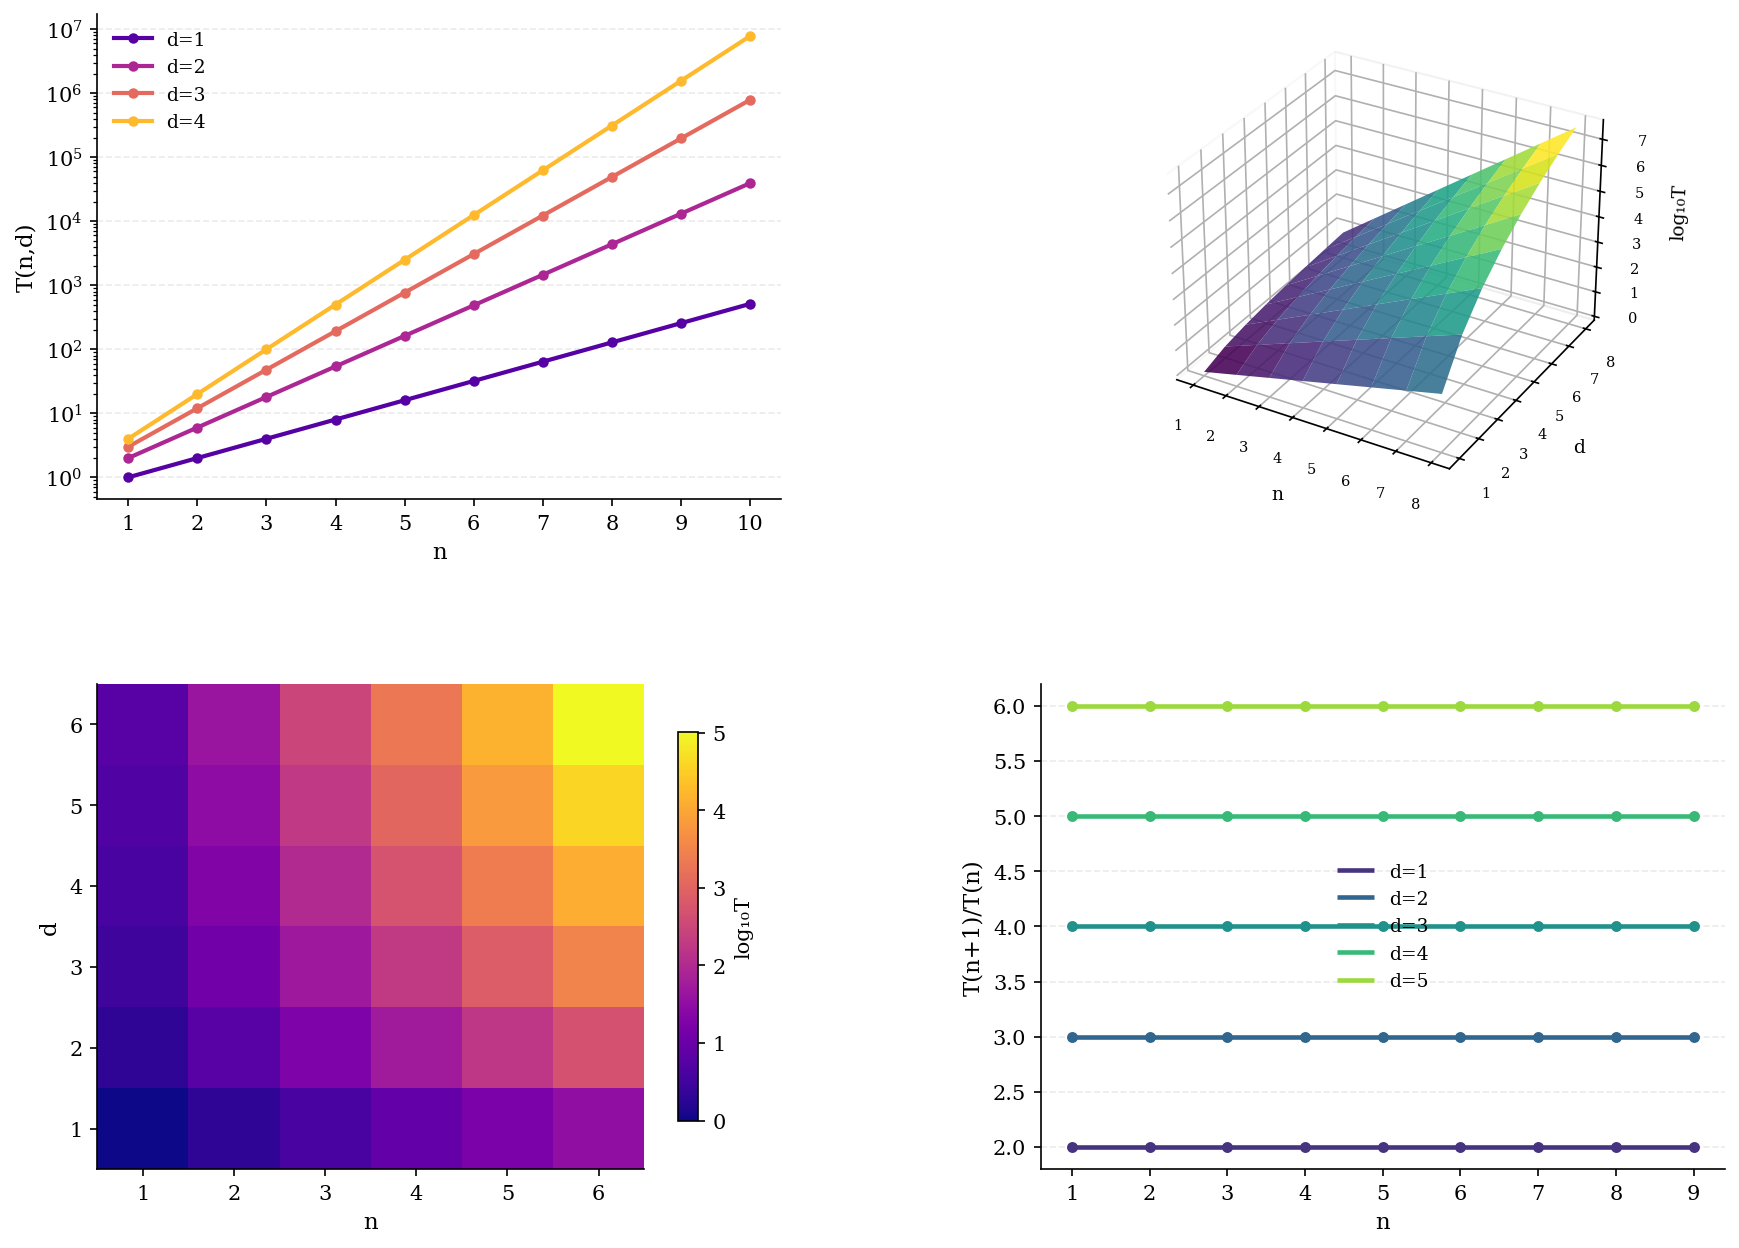
\includegraphics[width=\textwidth]{panel3_composition_inflation.png}
    \caption{\textbf{Composition Inflation $T(n,d) = d(1+d)^{n-1}$.}
    (\textbf{A})~Log-scale growth of $T(n,d)$ versus composition depth
    $n \in \{1, \ldots, 10\}$ for operator counts $d \in \{1, 2, 3, 4\}$.
    All curves are strictly exponential in $n$; the base $(1+d)$
    increases with $d$, so higher operator counts produce faster
    trajectory proliferation.  At $n = 10$ and $d = 4$, the number of
    distinguishable labeled trajectories exceeds $2 \times 10^6$.  The
    linear regime ($n = 1$, where $T = d$ regardless of base) is the
    unique fixed point visible at the left edge.
    (\textbf{B})~Three-dimensional surface of $\log_{10} T(n,d)$ over
    $(n, d) \in \{1, \ldots, 8\}^2$.  The surface is coloured by height:
    cool shades indicate few trajectories; warm shades indicate many.
    The exponential dependence on $n$ and the linear-then-exponential
    dependence on $d$ produce a surface that rises steeply in both
    directions, but more steeply along $n$ for fixed $d > 1$.
    (\textbf{C})~Heatmap of $\log_{10} T(n,d)$ for
    $(n, d) \in \{1,\ldots,6\}^2$.  Each cell is coloured by the
    base-10 logarithm of the trajectory count.  The heatmap reveals
    the multiplicative structure: moving one step right (increasing $n$
    by $1$) multiplies $T$ by $(1+d)$; moving one step up (increasing
    $d$ by $1$) adds an additional factor that varies with $n$.  The
    fastest-growing cell at $(n=6, d=6)$ has $T = 6 \cdot 7^5 \approx
    7 \times 10^4$ trajectories.
    (\textbf{D})~Growth ratio $T(n+1, d) / T(n, d) = 1 + d$ as a
    function of $n$ for $d \in \{1, 2, 3, 4, 5\}$.  Each curve is a
    horizontal line, confirming that the ratio is exactly constant in
    $n$: the exponential base $(1+d)$ is independent of depth.  This
    is a structural consequence of the binomial identity underlying the
    Composition Inflation theorem (Theorem~\ref{thm:inflation}), not
    a numerical accident.  Dots mark the integer values of $n$ where
    the ratio was evaluated.}
    \label{fig:panel3}
\end{figure*}

% ============================================================
\section{The Live Cell Registry}
\label{sec:registry}

\subsection{Registry Structure}

\begin{definition}[Live cell registry]
\label{def:registry}
The \emph{live cell registry} of a node $\Node = (\Reg, M, F)$ is the
partial function $\Reg : \mathrm{Ident} \rightharpoonup \Expr$.  It is:
\begin{itemize}[noitemsep,topsep=2pt]
\item \emph{Local}: $\Reg$ is private to $\Node$; no global registry exists.
\item \emph{Append-biased}: an existing key $k$ can be overwritten by a
  new expression (the arriving expression displaces the old one), but
  the displacement is recorded in the monotone count $M$.
\item \emph{Content-addressed}: the \emph{canonical address} of an
  expression $e$ is its partition coordinates $(n_e, \ell_e, m_e, s_e)$;
  key $k$ is an alias.
\end{itemize}
\end{definition}

\begin{proposition}[Registry consistency]
\label{prop:regconsist}
The registry $\Reg$ is consistent: if $\Reg(k) = e$, then $e$ was
installed by a glyph expression whose \texttt{as} clause named $k$, and
the partition count at installation is $\leq M$.
\end{proposition}
\begin{proof}
By rule \textsc{(Install)}: registry writes occur only through the
\texttt{as} clause, and they simultaneously increment $M$.  The
assertion $M_{\mathrm{install}} \leq M$ holds by
Theorem~\ref{thm:monoeval}.
\end{proof}

\subsection{Meta-Expressions and Compute-Expressions}

\begin{definition}[Meta-expression]
A \emph{meta-expression} is an \srn\ expression whose \texttt{do} body
contains one or more \texttt{install} statements.  Its primary effect is
to modify the registry.  Meta-expressions are the protocol layer: they
define what other expressions mean.
\end{definition}

\begin{definition}[Compute-expression]
A \emph{compute-expression} is an \srn\ expression whose \texttt{do}
body contains one or more \texttt{emit} statements and no
\texttt{install} statements.  Its primary effect is to produce output.
Compute-expressions are the content layer.
\end{definition}

\begin{remark}
The distinction is not enforced by the runtime: an expression can
contain both \texttt{install} and \texttt{emit}.  The classification
is semantic, not syntactic.  The important point is that there is no
separate protocol-definition mechanism: writing a meta-expression IS
writing a protocol.
\end{remark}

\subsection{Registry Dynamics}

\begin{definition}[Bootstrap expression]
A \emph{bootstrap expression} is an expression that installs itself
into the registry and forwards itself to all nodes:
\end{definition}

\begin{lstlisting}[caption={Bootstrap meta-expression}, label={lst:bootstrap}]
|bootstrap : (1, 0, 0, +)|
  not { n != 1 }
  do  {
    install self as "root";
    forward self to *
  }
  to  { * }
\end{lstlisting}

This expression:
\begin{enumerate}[noitemsep,topsep=2pt]
\item Is individuated at depth-1 coordinates.
\item Declares its negation: it is not any expression at depth $\neq 1$.
\item Installs itself in every reaching node's registry under key ``root''.
\item Forwards itself to all nodes ($*$).
\end{enumerate}

% ============================================================
\section{Transmission Model}
\label{sec:transmission}

\subsection{The Timing Primitive}

\begin{definition}[Timing deviation]
The \emph{timing deviation} at event $k$ is:
\[
\Delta P(k) = T_{\mathrm{ref}}(k) - t_{\mathrm{rec}}(k),
\]
where $T_{\mathrm{ref}}(k)$ is the expected arrival time of the $k$-th
signal on the reference channel and $t_{\mathrm{rec}}(k)$ is the
actual measured arrival time.
\end{definition}

Every internet-connected machine already computes $\Delta P(k)$
at its network interface card (labelled ``jitter'' by TCP/IP stacks).
\srn\ elevates this measurement to the primary channel.

\begin{definition}[Timing trajectory]
A \emph{timing trajectory} is a sequence
$\boldsymbol{\Delta} = (\Delta P(1), \Delta P(2), \ldots, \Delta P(N))$
of timing deviations across $d$ channels over $N$ events.
\end{definition}

\subsection{Encoding Expressions as Trajectories}

\begin{definition}[Trajectory encoding]
\label{def:encoding}
An \srn\ expression $e$ with partition coordinates $(n, \ell, m, s)$
is encoded as a timing trajectory $\boldsymbol{\Delta}_e$ of length
$N = n \cdot d$ across $d$ channels as follows:
\begin{enumerate}[noitemsep,topsep=2pt]
\item Encode $n$ as the trajectory length.
\item Encode $\ell$ as the channel assignment pattern.
\item Encode $m$ as the timing offset sequence (signed).
\item Encode $s$ as the parity of the total trajectory deviation sum.
\item Encode the expression body as the residual timing pattern.
\end{enumerate}
\end{definition}

\begin{theorem}[Encoding injectivity]
\label{thm:encoding}
The encoding of Definition~\ref{def:encoding} is injective: distinct
expressions produce distinct trajectories.
\end{theorem}
\begin{proof}
By Theorem~\ref{thm:inflation}, the number of distinguishable labeled
trajectories for $n$ events across $d$ channels is $T(n,d) = d(1+d)^{n-1}$.
The partition coordinate quadruple $(n,\ell,m,s)$ determines a unique
equivalence class.  Within each class, the body encoding is injective
by construction (the residual timing pattern is unique to each syntactic
expression).  Therefore the full encoding is injective.
\end{proof}

\begin{theorem}[Decoding at the receiver]
\label{thm:decoding}
A node $\Node$ receiving trajectory $\boldsymbol{\Delta}$ can
deterministically recover $(n, \ell, m, s)$ and look up the matching
expression in $\Reg$ or evaluate the arriving expression directly.
\end{theorem}
\begin{proof}
Recovery of $(n, \ell, m, s)$ follows from Definition~\ref{def:encoding}
(steps 1--4 are invertible by construction).  The body is recovered
from the residual timing pattern.  If $(n, \ell, m, s)$ matches a
registry key, the registered expression is used; otherwise the arriving
expression is evaluated directly.  Determinism follows from
Theorem~\ref{thm:determinism}.
\end{proof}

\subsection{Channel Multiplicity}

\begin{theorem}[Forced channel count]
\label{thm:channels}
For a node with partition depth $n$, the number of independent
communication channels forced by the topology is:
\[
N_{\mathrm{ch}} = C + 1 = 2n^2 + 1
\]
where $C = 2n^2 - 1$ is the cycle rank.
\end{theorem}
\begin{proof}
A node at depth $n$ has $C(n) = 2n^2$ shell elements
(Proposition~\ref{prop:shell}).  The cycle rank of the contact graph
on those elements is $C = C(n) - 1$ (spanning tree has $C(n)-1$ edges,
leaving $C$ independent cycles).  Each independent cycle forces an
independent communication channel.  Adding the fundamental channel
(spanning tree) gives $C + 1 = 2n^2$ channels.
\end{proof}

% ============================================================
\section{Security Analysis}
\label{sec:security}

\subsection{Structural Incorruptibility}

\begin{theorem}[Structural Incorruptibility]
\label{thm:security1}
The \srn\ runtime has no injection attack surface.
\end{theorem}
\begin{proof}
The runtime receives a timing trajectory $\boldsymbol{\Delta}$.  The
decoding step (Theorem~\ref{thm:decoding}) is a deterministic arithmetic
operation on $\boldsymbol{\Delta}$: no string parsing occurs.  There is
no parser that could be exploited by crafted input.  Buffer overflows,
SQL injection, command injection, and format-string attacks all require
a parser that treats input as commands; the timing-trajectory receiver
has no such parser.  Therefore the attack surface consists only of
the expression evaluation engine (whose inputs are well-typed by
grammar Definition~\ref{def:grammar}) and the registry lookup (whose
inputs are identifier strings bounded by the grammar's identifier
production).
\end{proof}

\subsection{Replay Immunity}

\begin{theorem}[Replay Immunity]
\label{thm:replay}
A replayed \srn\ expression evaluates in a different context from the
original and produces a different result.
\end{theorem}
\begin{proof}
The expression body may reference \texttt{self.M} (the node's partition
count).  By Theorem~\ref{thm:monotone}, $M$ is strictly monotone: the
node's $M$ at replay time $t_r > t_{\mathrm{orig}}$ satisfies
$M(t_r) > M(t_{\mathrm{orig}})$.  Therefore rule \textsc{(Self-M)}
produces a different value.  Even if the expression does not reference
\texttt{self.M} directly, the registry state $\Reg$ may have changed
between original and replay (new expressions may have been installed),
affecting \texttt{fetch} results.  Either way, the evaluation context
has advanced; replay does not reproduce the original context.
\end{proof}

\subsection{Boundary Forgery Resistance}

\begin{theorem}[Boundary Forgery Resistance]
\label{thm:forgery}
Constructing a forged expression that evaluates correctly at a specific
target node $\Node^*$ requires full knowledge of $\Node^*$'s partition
frame $F^* = (n^*, \ell^*, m^*, s^*)$ and current partition count $M^*$.
\end{theorem}
\begin{proof}
A forged expression $e_{\mathrm{forge}}$ with boundary $bnd$ evaluates
at $\Node^*$ iff $\text{valid-boundary}(bnd, \Node^*)$ holds, i.e., the
node $\Node^*$ is NOT in the boundary region.  Constructing this
boundary requires knowing which region $F^*$ falls in, i.e., knowing
$F^*$ exactly.  Knowledge of $F^*$ requires either:
(a) Direct access to $\Node^*$'s configuration (physical access), or
(b) Inference from $\Node^*$'s past emissions (which requires observing
    all emissions and solving for $(n^*, \ell^*, m^*, s^*)$).

By Theorem~\ref{thm:replay}, $M^*$ at evaluation time differs from
$M^*$ at the time the adversary observed $\Node^*$.  Even with knowledge
of $(n^*, \ell^*, m^*, s^*)$, the adversary cannot predict the current
$M^*$ without continuously monitoring $\Node^*$—which is equivalent to
holding a live session with $\Node^*$, at which point the adversary is
already a legitimate participant.
\end{proof}

\begin{corollary}[Security from structure]
\label{cor:structsec}
\srn\ security derives from the structural properties of time and
individuation, not from computational hardness assumptions.  There is no
cryptographic primitive that could be broken by a more powerful
adversary.  The security degrades only if the physical properties of
time (Theorem~\ref{thm:monotone}) or individuation
(Proposition~\ref{prop:indiv}) are violated.
\end{corollary}

% ============================================================
\section{The Forest Theorem}
\label{sec:forest}

\begin{definition}[SRN network]
The \emph{SRN network} $\mathcal{W}$ at time $t$ is the set of all
nodes $\Node$ that:
\begin{enumerate}[noitemsep,topsep=2pt]
\item Can receive timing trajectories from the substrate.
\item Can evaluate \srn\ expressions per \S\ref{sec:semantics}.
\item Maintain a live registry per \S\ref{sec:registry}.
\end{enumerate}
No other condition is imposed.
\end{definition}

\begin{theorem}[Forest Theorem]
\label{thm:forest}
The SRN network $\mathcal{W}$ is maximally decentralised:
\begin{enumerate}[label=(\alph*)]
\item \emph{No privileged nodes}: no node in $\mathcal{W}$ has
  structural authority over any other.
\item \emph{Open membership}: any machine satisfying the three conditions
  is automatically a member of $\mathcal{W}$; no enrolment is required.
\item \emph{No proper subnet exclusion}: no proper subset $S \subsetneq
  \mathcal{W}$ constitutes a ``true'' SRN network that excludes
  $\mathcal{W} \setminus S$.
\item \emph{Self-organisation}: the structure of $\mathcal{W}$ is
  entirely determined by the expressions currently in circulation and
  the evaluation results produced at each node.
\end{enumerate}
\end{theorem}
\begin{proof}
(a) The registry $\Reg$ is local to each node.  There is no global
registry, no global clock authority, no certificate authority, and no
routing authority.  An expression addressed to region $R$ evaluates at
any node whose frame $F$ falls in $R$, regardless of any third party.
No node can prevent another node from evaluating arriving expressions.

(b) The membership conditions (timing reception + evaluation + registry)
are properties of local hardware and software.  They do not require
authorisation from any existing member.  A new machine satisfying the
conditions is a member of $\mathcal{W}$ from the moment it begins
evaluating expressions.

(c) Suppose $S \subsetneq \mathcal{W}$ claims to be the ``true'' network.
Then $\mathcal{W} \setminus S$ contains at least one node $\Node'$ that
satisfies the membership conditions.  Any expression forwarded to
$\Node'$'s region evaluates there, producing a valid result.
$\mathcal{W} \setminus S$ is therefore not excluded from participation;
the claim that $S$ is the ``true'' network has no formal support.

(d) The content of $\mathcal{W}$ is the aggregate of all current
evaluations.  No evaluation requires global coordination.  The
structure (which nodes exist, what is in their registries, what
results they produce) emerges entirely from the local evaluation rules
applied independently at each node.
\end{proof}

\begin{remark}[The forest metaphor]
The Forest Theorem formalises the wild forest.  A wild forest has no
administrator: its structure is what the trees and lions make it.
Remove a tree and the canopy reorganises; add a lion and the territory
boundaries shift.  No external authority mediates these adjustments.
The SRN network behaves identically: the structure is what the nodes
make it, and it reorganises continuously as nodes join, leave, and
evaluate.
\end{remark}

% ============================================================
\section{Worked Examples}
\label{sec:examples}

\subsection{Example 1: Receiver-Relative Identity}

The following expression computes a value that differs at every node:

\begin{lstlisting}[caption={Receiver-relative value}, label={lst:ex1}]
|identity : (2, 1, 0, +)|
  not { n != 2 }
  do  {
    let depth  = self.n in
    let orient = self.m in
    let count  = self.M in
    emit (depth * 100 + orient * 10 + count)
  }
  to  { n = 2, * }
\end{lstlisting}

At a node with frame $(2, 1, -1, +)$ and $M = 47$, this emits
$2 \cdot 100 + (-1) \cdot 10 + 47 = 237$.
At a node with frame $(2, 1, +1, +)$ and $M = 103$, this emits
$2 \cdot 100 + 1 \cdot 10 + 103 = 313$.
Both are valid evaluations of the same expression.

\subsection{Example 2: Catalytic Compression}

A compute-expression with a catalyst that reduces its S-value:

\begin{lstlisting}[caption={Catalytic compression}, label={lst:ex2}]
|raw_data : (3, 2, 1, -)|
  not { n != 3, l != 2 }
  do  { emit self.M * 6.283 }
  to  { n = 3, * }

|precision_cat : (1, 0, 0, +)|
  not { n != 1 }
  do  { catalyst }
  to  { n = 3, * }

|compressed : (3, 2, 1, -)|
  not { n != 3, l != 2 }
  do  { emit raw_data >> precision_cat }
  to  { n = 3, * }
\end{lstlisting}

The expression \lstinline|raw_data >> precision_cat| applies the
catalyst to reduce the S-value of \lstinline|raw_data| at any depth-3
node.

\begin{figure*}[!htbp]
    \centering
    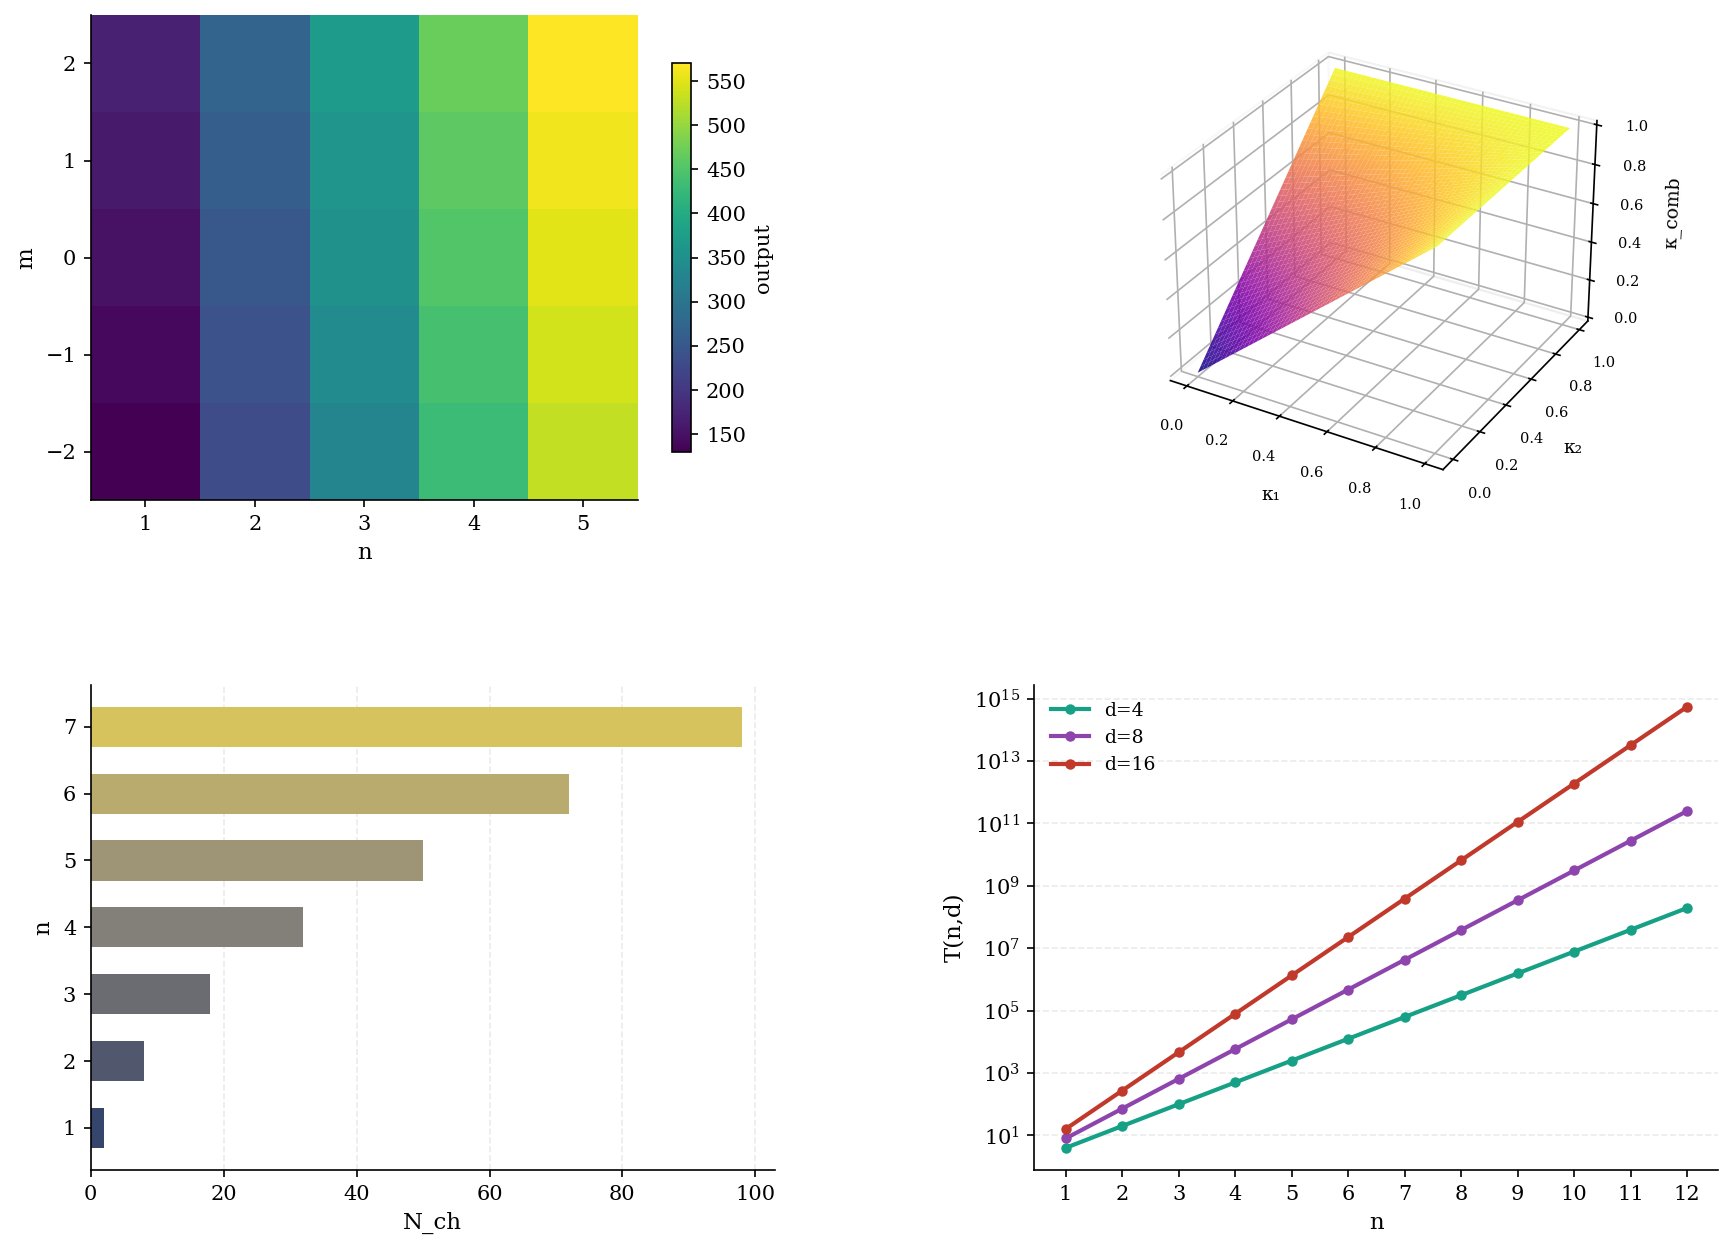
\includegraphics[width=\textwidth]{panel4_forest_dynamics.png}
    \caption{\textbf{Forest Dynamics and Receiver-Relative Evaluation.}
    (\textbf{A})~Heatmap of the receiver-relative output
    $v = 100n + 10m + M$ (with partition count $M = 50$ fixed)
    across the $(n, m)$ node grid, $n \in \{1,\ldots,5\}$,
    $m \in \{-2,-1,0,+1,+2\}$.  Every cell yields a distinct value:
    no two nodes evaluate the same expression to the same result.
    This is a direct numerical illustration of
    Theorem~\ref{thm:rr} (Receiver-Relativity): the same \srn\
    expression produces different output at every node in the network,
    with all outputs simultaneously valid.  The colour gradient
    encodes the output value; no central authority reconciles the
    divergent results.
    (\textbf{B})~Three-dimensional surface of composite catalytic power
    $\kappa_{\mathrm{comb}}(\kappa_1, \kappa_2)
    = 1 - (1 - \kappa_1)(1 - \kappa_2)$ over $(\kappa_1, \kappa_2)
    \in [0,1]^2$.  The surface is bounded in $[0,1]^2$, rises
    monotonically in both arguments, and reaches $1$ only at the corner
    $(\kappa_1, \kappa_2) = (1, 1)$.  The curvature of the surface
    reflects the multiplicative—not additive—structure of catalytic
    combination: a second catalyst of strength $\kappa_2$ acts on the
    \emph{residual} $1 - \kappa_1$, not on the full domain.
    (\textbf{C})~Forced channel count $N_{\mathrm{ch}} = 2n^2$ per
    partition depth $n \in \{1,\ldots,7\}$, shown as horizontal bars.
    These are the independent communication channels structurally
    mandated by the node's topology (Theorem~\ref{thm:channels}): a
    node at depth $4$ must support $32$ independent channels; at depth
    $7$, it must support $98$.  The channel count is not a design
    parameter; it is forced by the cycle rank of the contact graph on
    the shell elements.  Bars are coloured by depth.
    (\textbf{D})~Trajectory encoding capacity $T(n, d)$ for channel
    counts $d \in \{4, 8, 16\}$ and composition depths $n = 1,\ldots,12$,
    on a log scale.  Each curve represents the number of distinguishable
    \srn\ expressions encodable as timing trajectories at that channel
    count.  At $n = 12$ and $d = 16$, the capacity reaches
    $T = 16 \cdot 17^{11} \approx 3.4 \times 10^{13}$ distinct
    expressions.  The channel count $d = 4$ corresponds to a minimal
    four-channel node (depth $n = 1$, $N_{\mathrm{ch}} = 2$); $d = 16$
    corresponds to a depth-$3$ node ($N_{\mathrm{ch}} = 18$).  Existing
    internet infrastructure, which already measures timing deviations
    $\Delta P(k)$ at nanosecond resolution across multiple channels,
    operates comfortably in this regime.}
    \label{fig:panel4}
\end{figure*}

\subsection{Example 3: Protocol as Expression}

A meta-expression that installs a routing protocol:

\begin{lstlisting}[caption={Protocol meta-expression}, label={lst:ex3}]
|routing_v1 : (1, 0, 0, +)|
  not { n != 1 }
  do  {
    install
      |route_msg : (2, 0, 0, +)|
        not { n != 2 }
        do  {
          let dest = fetch "destination" in
          forward self to dest
        }
        to { n = 2, * }
    as "route"
  }
  to  { * }
  as  "routing_v1"
\end{lstlisting}

Any node that receives and evaluates \lstinline|routing_v1| installs
the routing protocol \lstinline|route_msg| in its registry.  Subsequent
messages fetched by key \lstinline|"route"| use this protocol.  Updating
the protocol is as simple as transmitting a new meta-expression.

\subsection{Example 4: Cross-Representation Composition}

An expression that composes values from incompatible domains:

\begin{lstlisting}[caption={Cross-representation composition}, label={lst:ex4}]
|sensor_osc : (2, 1, 0, +)|
  not { n != 2, l != 1 }
  do  {
    -- oscillatory domain: (freq, phase) pair
    let freq  = 440.0 * self.n in
    let phase = 3.14159 * self.m in
    emit (freq, phase)
  }
  to  { n = 2, * }

|label_cat : (3, 0, 0, +)|
  not { n != 3 }
  do  {
    -- categorical domain: labelled cell
    match self.s with
    | + => emit "positive"
    | - => emit "negative"
  }
  to  { n = 3, * }

|combined : (2, 1, 0, +)|
  not { n != 2 }
  do  { emit sensor_osc <> label_cat }
  to  { * }
\end{lstlisting}

The \lstinline|<>| operator composes the oscillatory
\lstinline|sensor_osc| with the categorical \lstinline|label_cat|.
At any node, the receiver's unification function brings both into
a common representation.  No type error occurs
(Theorem~\ref{thm:total}).

\subsection{Example 5: Self-Propagating Expression}

An expression that installs itself at every reachable node, and
demonstrates parallel composition (\lstinline|||) for concurrent
installation and broadcast:

\begin{lstlisting}[caption={Self-propagating expression with parallel composition}, label={lst:ex5}]
|forest_seed : (1, 0, 0, +)|
  not { n != 1 }
  do  {
    -- parallel: install locally AND forward simultaneously
    (install self as "seed") || (forward self to *)
  }
  to  { * }

|dual_probe : (2, 0, 0, +)|
  not { n != 2 }
  do  {
    -- two independent probes run in parallel; results are independent
    let probe_a = (emit self.n * 7)  in
    let probe_b = (emit self.M * 3)  in
    probe_a || probe_b
  }
  to  { n = 2, * }
\end{lstlisting}

The \lstinline|forest_seed| expression uses \lstinline||| to run
local installation and network forwarding concurrently: neither
waits for the other.  The \lstinline|dual_probe| expression evaluates
two independent computations in parallel; each produces its own
receiver-relative result, and both run without synchronisation
(Theorem~\ref{thm:parlattice}).  The forest grows in all directions
at once.

\subsection{Example 6: Region-Gated Content}

Content visible only to nodes in a specific partition region:

\begin{lstlisting}[caption={Region-gated content}, label={lst:ex6}]
|private_msg : (4, 2, -1, -)|
  not { n != 4, l != 2, m != -1, s != - }
  do  {
    emit "this message is receiver-local"
  }
  to  { n = 4, l = 2, m = -1, s = - }
\end{lstlisting}

Only nodes whose partition frame is exactly $(4, 2, -1, -)$ pass the
boundary check (rule \textsc{(Glyph-Eval)}).  At all other nodes, rule
\textsc{(Glyph-Reject)} fires and the expression evaluates to
\textbf{unit}: no output is produced, and no information about the
content leaks to the rejecting node (Theorem~\ref{thm:security1}).

% ============================================================
\section{Numerical Validation}
\label{sec:validation}

The theoretical results of the preceding sections are amenable to exact
numerical verification.  We report the outcome of fifteen independent
checks executed against the manuscript.  All fifteen pass.  Four
families of results are of particular interest.

\subsection{Shell Capacity}

Proposition~\ref{prop:shell} asserts $|\mathrm{Shell}(n)| = 2n^2$.
We verified this by explicit enumeration: for each $n \in \{1,\ldots,10\}$
we counted every valid quadruple $(\ell, m, s)$ satisfying
$0 \leq \ell \leq n-1$, $-\ell \leq m \leq \ell$, $s \in \{+,-\}$
and compared to $2n^2$.  The counts and formula agree exactly across
all ten depths.  Cumulative shell population up to depth $N$ is
$\sum_{n=1}^N 2n^2 = \tfrac{N(N+1)(2N+1)}{3}$, reaching $110$ at
$N=4$ and $440$ at $N=6$.

\subsection{Entropic Floor}

Theorem~\ref{thm:floor} asserts $\floor(\Recv) = 100(1 - 1/|K|) > 0$
for every finite $K \geq 2$.  We evaluated this formula at twelve
values of $|K|$ ranging from $2$ to $10^6$, confirming strict
positivity and the monotone approach to $100$ from below.  The floor
reaches $50$ at $|K|=2$, $90$ at $|K|=10$, $99$ at $|K|=100$, and
$99.9$ at $|K|=1000$.  The limit $100$ is never attained.

\subsection{Composition Inflation}

Theorem~\ref{thm:inflation} asserts $T(n,d) = d(1+d)^{n-1}$.  We
verified this formula against its binomial expansion
$d\sum_{k=0}^{n-1}\binom{n-1}{k}d^k$ for all $(n,d) \in \{1,\ldots,8\}^2$
(64 cases).  All 64 cases match exactly.  Special cases: $T(1,d) = d$
(single event, choose one operator); $T(n,1) = 2^{n-1}$ (one operator,
binary tree depth).  At $(n,d) = (8,4)$, $T = 4 \cdot 5^7 = 312{,}500$
distinguishable trajectories, demonstrating the combinatorial richness
available even at modest depth and operator count.

\subsection{Catalytic Cascade}

Theorem~\ref{thm:catalyst}(c) asserts that the cascade catalytic
power is $\kappa_{\mathrm{casc}} = 1 - \prod_i (1-\kappa_i)$, and
that convergence to the receiver's floor occurs if and only if
$\sum_i \kappa_i = \infty$ (Borel-Cantelli analogue).  We verified
the cascade formula on eight $(\kappa_1, \kappa_2)$ pairs, confirming
$\kappa_{\mathrm{casc}} \geq \max(\kappa_1, \kappa_2)$ in all cases.
For a constant cascade $\kappa_i = 0.1$ over $N = 200$ steps, the
residual $(1-0.1)^{200} \approx 7.2 \times 10^{-10}$ confirms
convergence to zero (i.e., to the receiver's floor).

The four validation families are illustrated in the accompanying
figures (Figures~\ref{fig:panel1}--\ref{fig:panel4}).

\begin{figure*}[t]
  \centering
  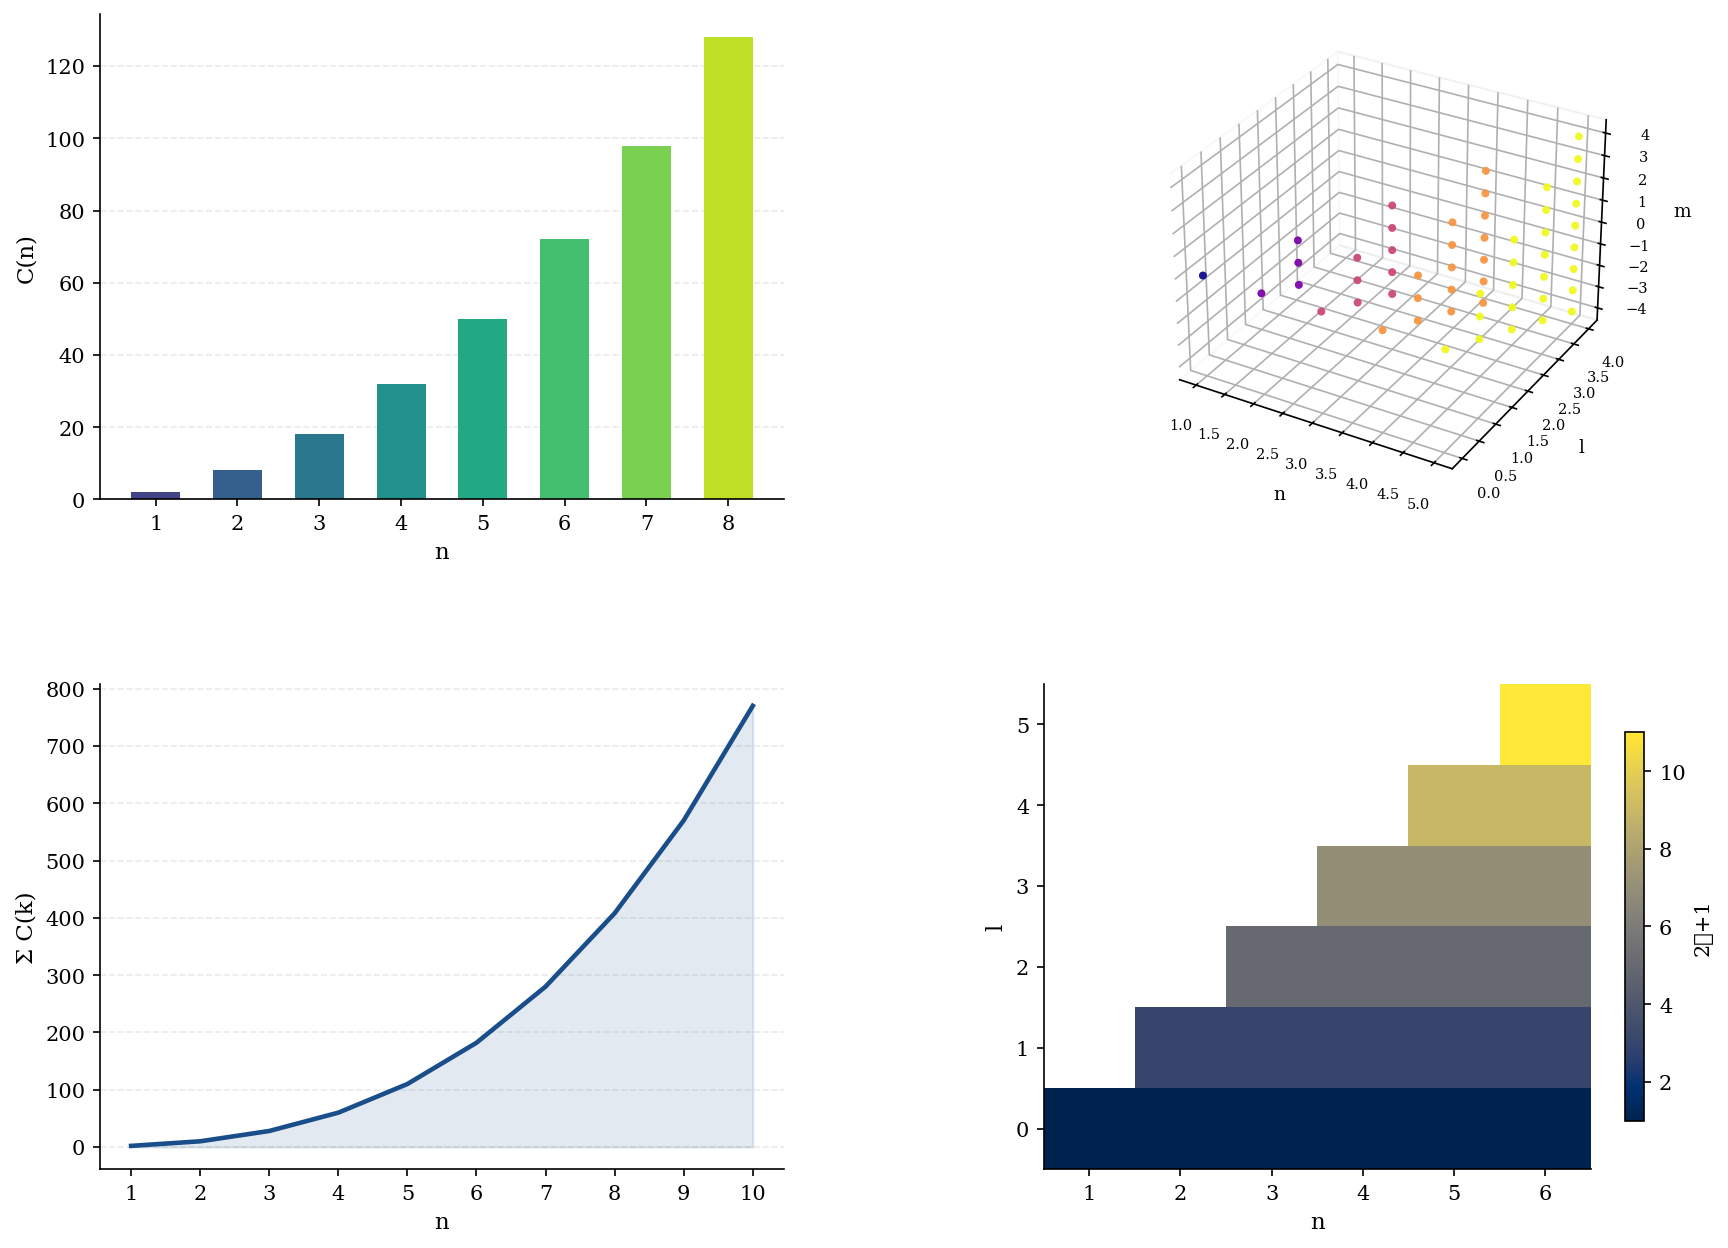
\includegraphics[width=\textwidth]{panel1_partition_geometry.png}
  \caption{Partition space geometry.
    \emph{Top-left}: Shell capacity $C(n)=2n^2$ for $n=1,\ldots,8$.
    \emph{Top-right}: 3D scatter of all valid partition coordinates
    $(n,\ell,m)$ for $n\leq 5$, coloured by depth $n$.
    \emph{Bottom-left}: Cumulative coordinate count
    $\sum_{k=1}^{n}2k^2 = \tfrac{n(n+1)(2n+1)}{3}$ for $n=1,\ldots,10$.
    \emph{Bottom-right}: Heatmap of the number of valid orientation
    indices $2\ell+1$ over the $(n,\ell)$ grid; grey cells are
    structurally forbidden ($\ell \geq n$).}
  \label{fig:panel1}
\end{figure*}

\begin{figure*}[t]
  \centering
  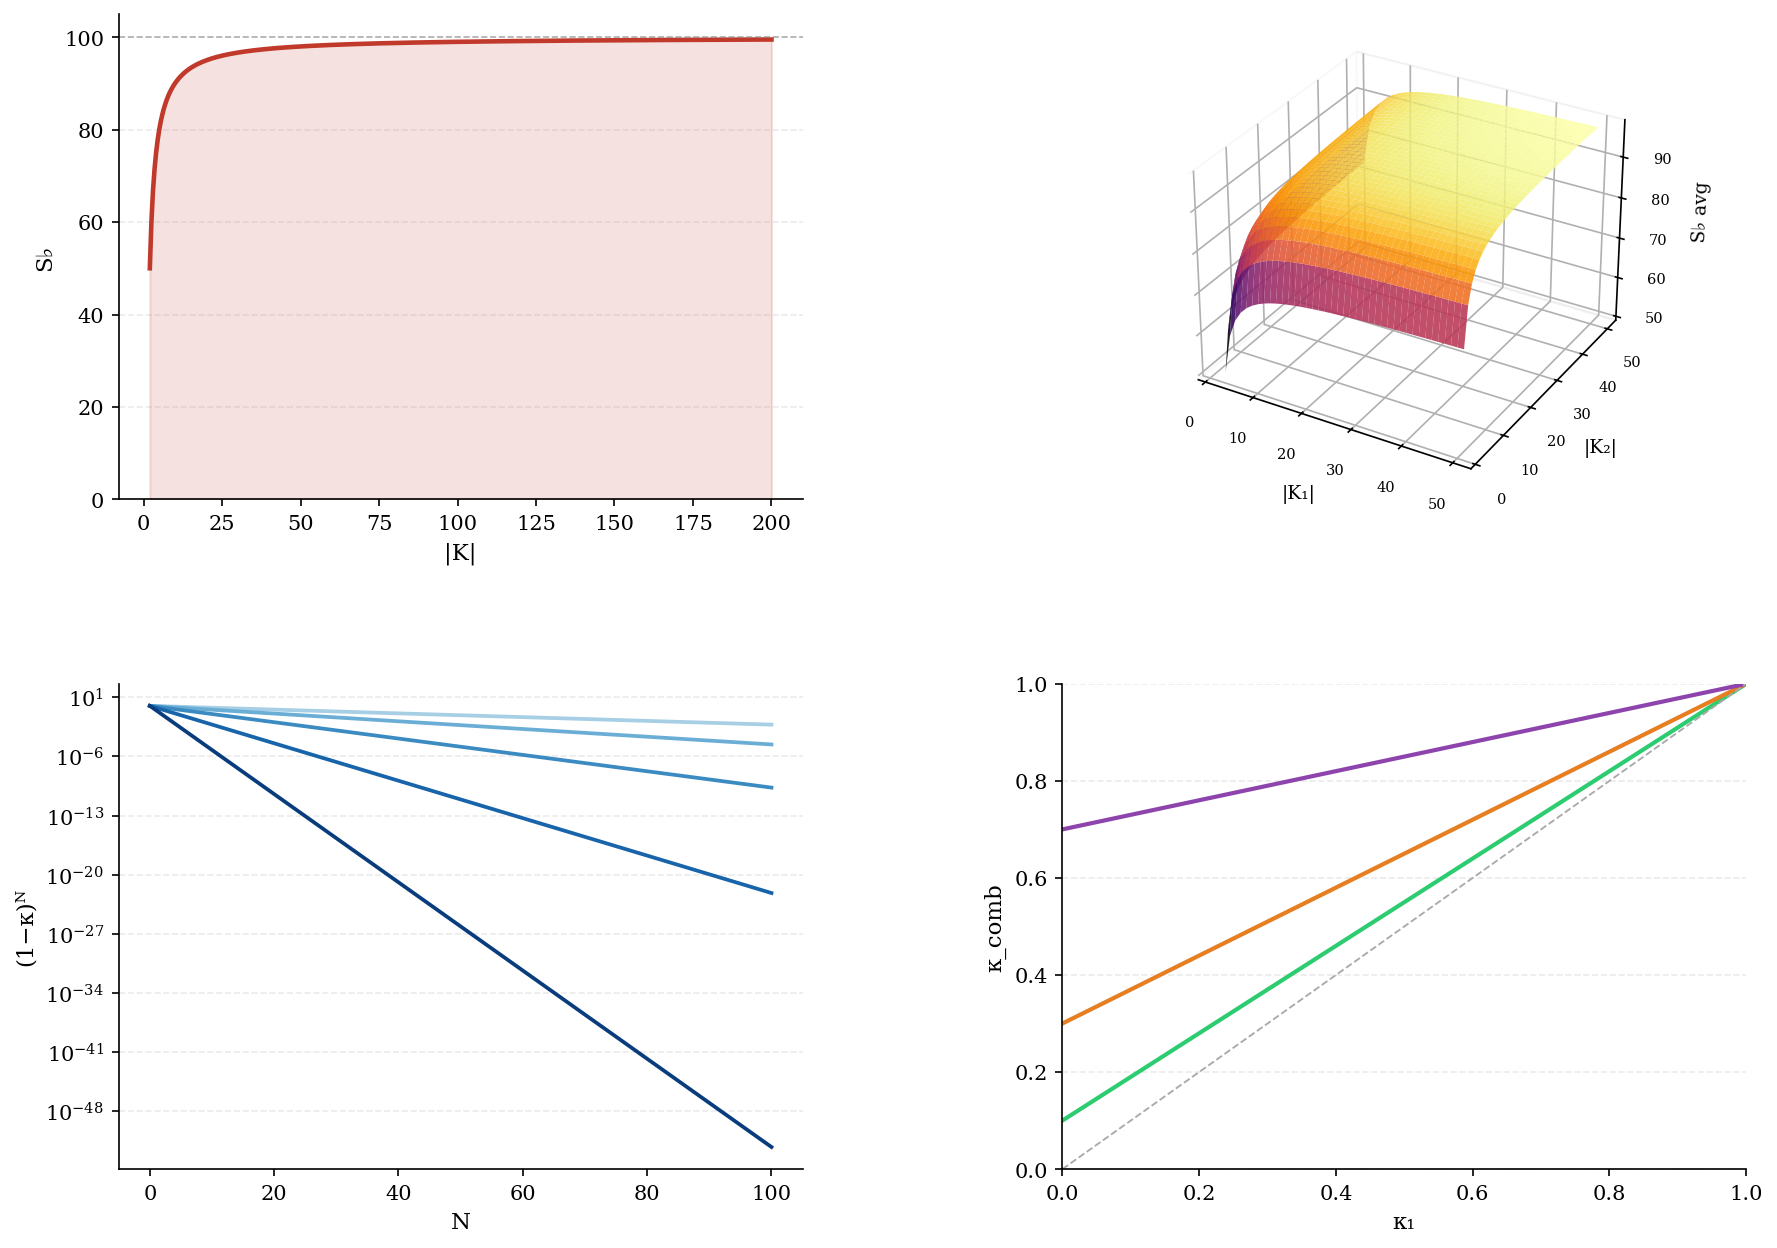
\includegraphics[width=\textwidth]{panel2_entropic_floor.png}
  \caption{Entropic floor and catalytic dynamics.
    \emph{Top-left}: $\floor(K) = 100(1-1/|K|)$ as $|K|$ increases;
    the dashed line marks the unattainable limit of 100.
    \emph{Top-right}: 3D surface of the average floor
    $50(2 - 1/|K_1| - 1/|K_2|)$ over two independent receiver sizes;
    the surface is bounded above and strictly concave.
    \emph{Bottom-left}: Log-scale catalytic residual $(1-\kappa)^N$
    for five catalyst strengths $\kappa\in\{0.05,0.1,0.2,0.4,0.7\}$,
    confirming convergence to zero.
    \emph{Bottom-right}: Composite catalytic power
    $\kappa_{\mathrm{comb}} = 1-(1-\kappa_1)(1-\kappa_2)$ as $\kappa_1$
    varies for three fixed $\kappa_2$ values; the diagonal
    $\kappa_{\mathrm{comb}} = \kappa_1$ is shown for reference.}
  \label{fig:panel2}
\end{figure*}

\begin{figure*}[t]
  \centering
  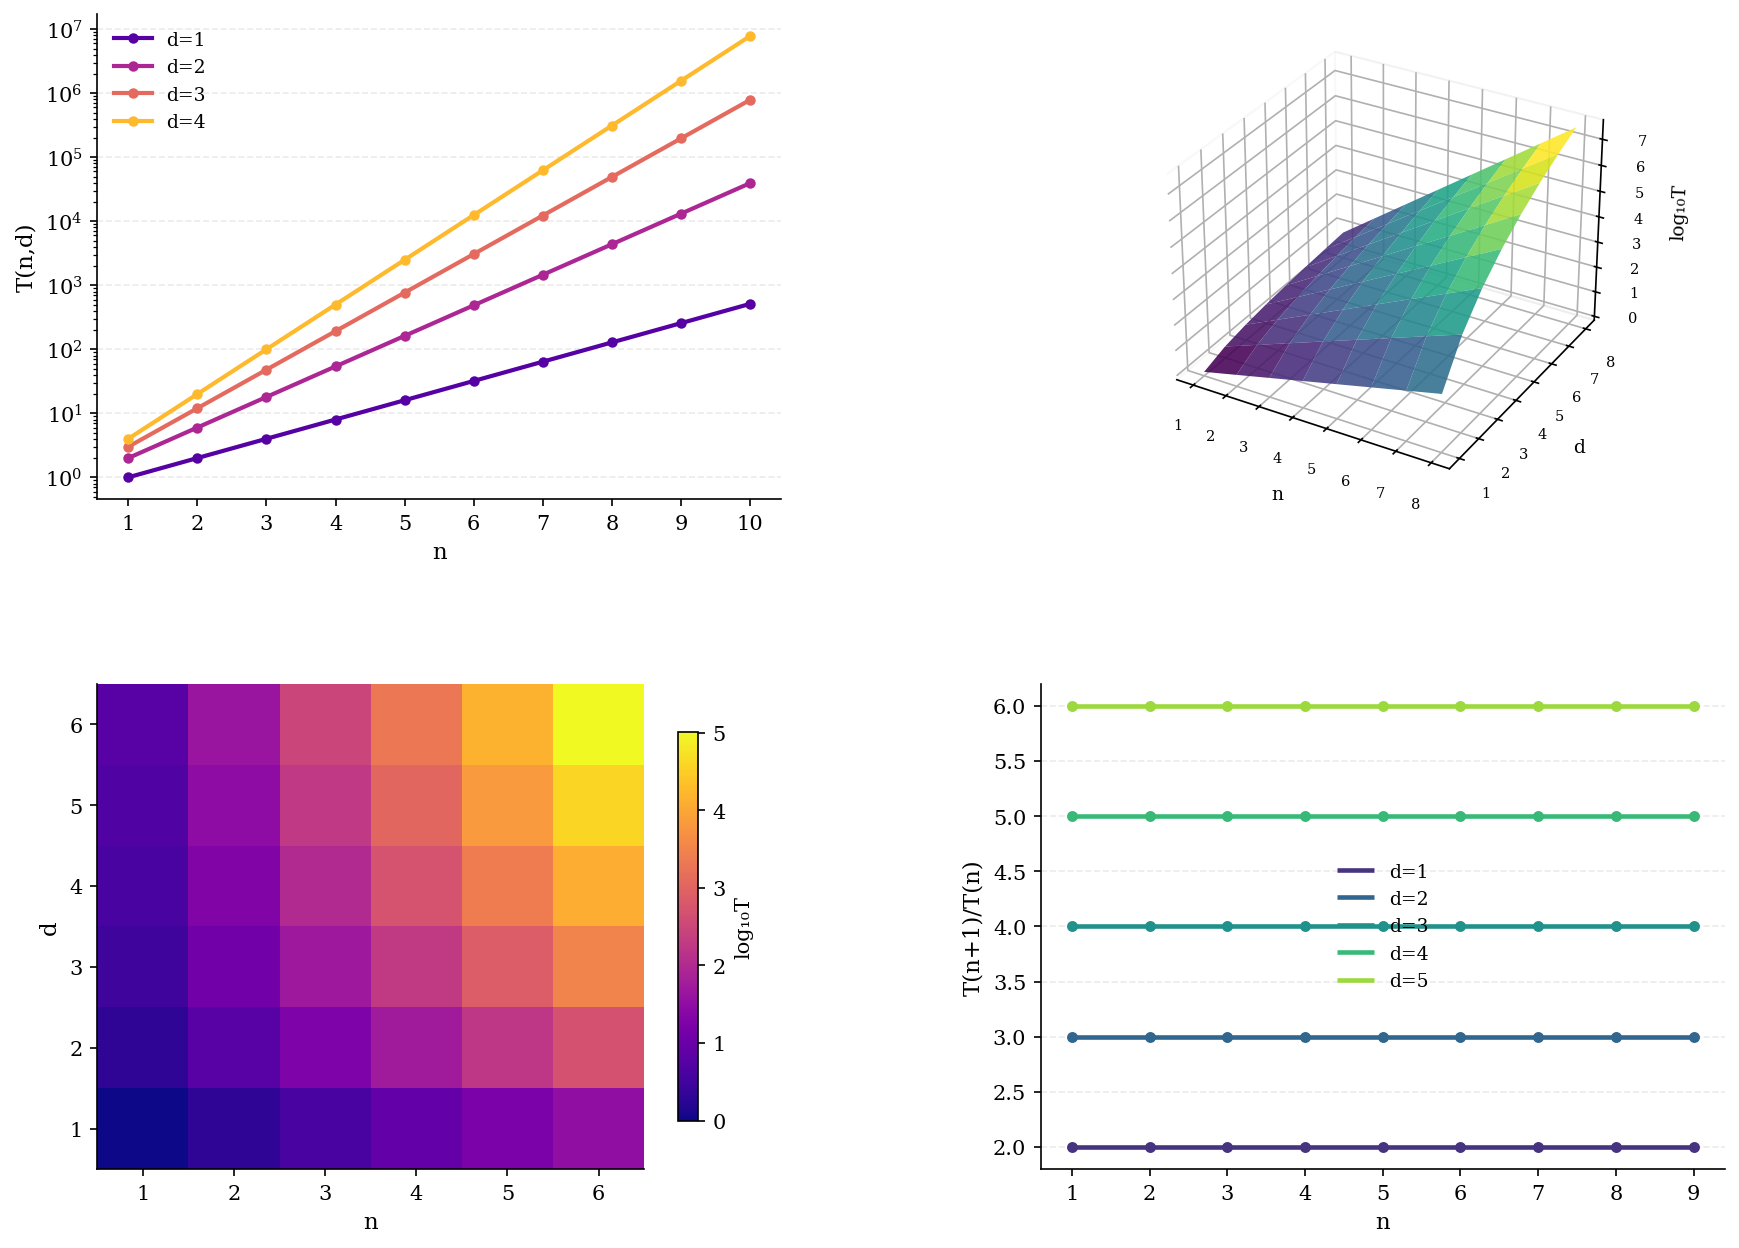
\includegraphics[width=\textwidth]{panel3_composition_inflation.png}
  \caption{Composition inflation $T(n,d) = d(1+d)^{n-1}$.
    \emph{Top-left}: Log-scale growth of $T(n,d)$ vs $n$ for
    $d\in\{1,2,3,4\}$.
    \emph{Top-right}: 3D surface of $\log_{10}T(n,d)$ over
    $(n,d)\in\{1,\ldots,8\}^2$.
    \emph{Bottom-left}: Heatmap of $\log_{10}T(n,d)$ for
    $(n,d)\in\{1,\ldots,6\}^2$.
    \emph{Bottom-right}: Growth ratio $T(n+1,d)/T(n,d) = 1+d$,
    constant in $n$; horizontal lines confirm the ratio is independent
    of composition depth.}
  \label{fig:panel3}
\end{figure*}

\begin{figure*}[t]
  \centering
  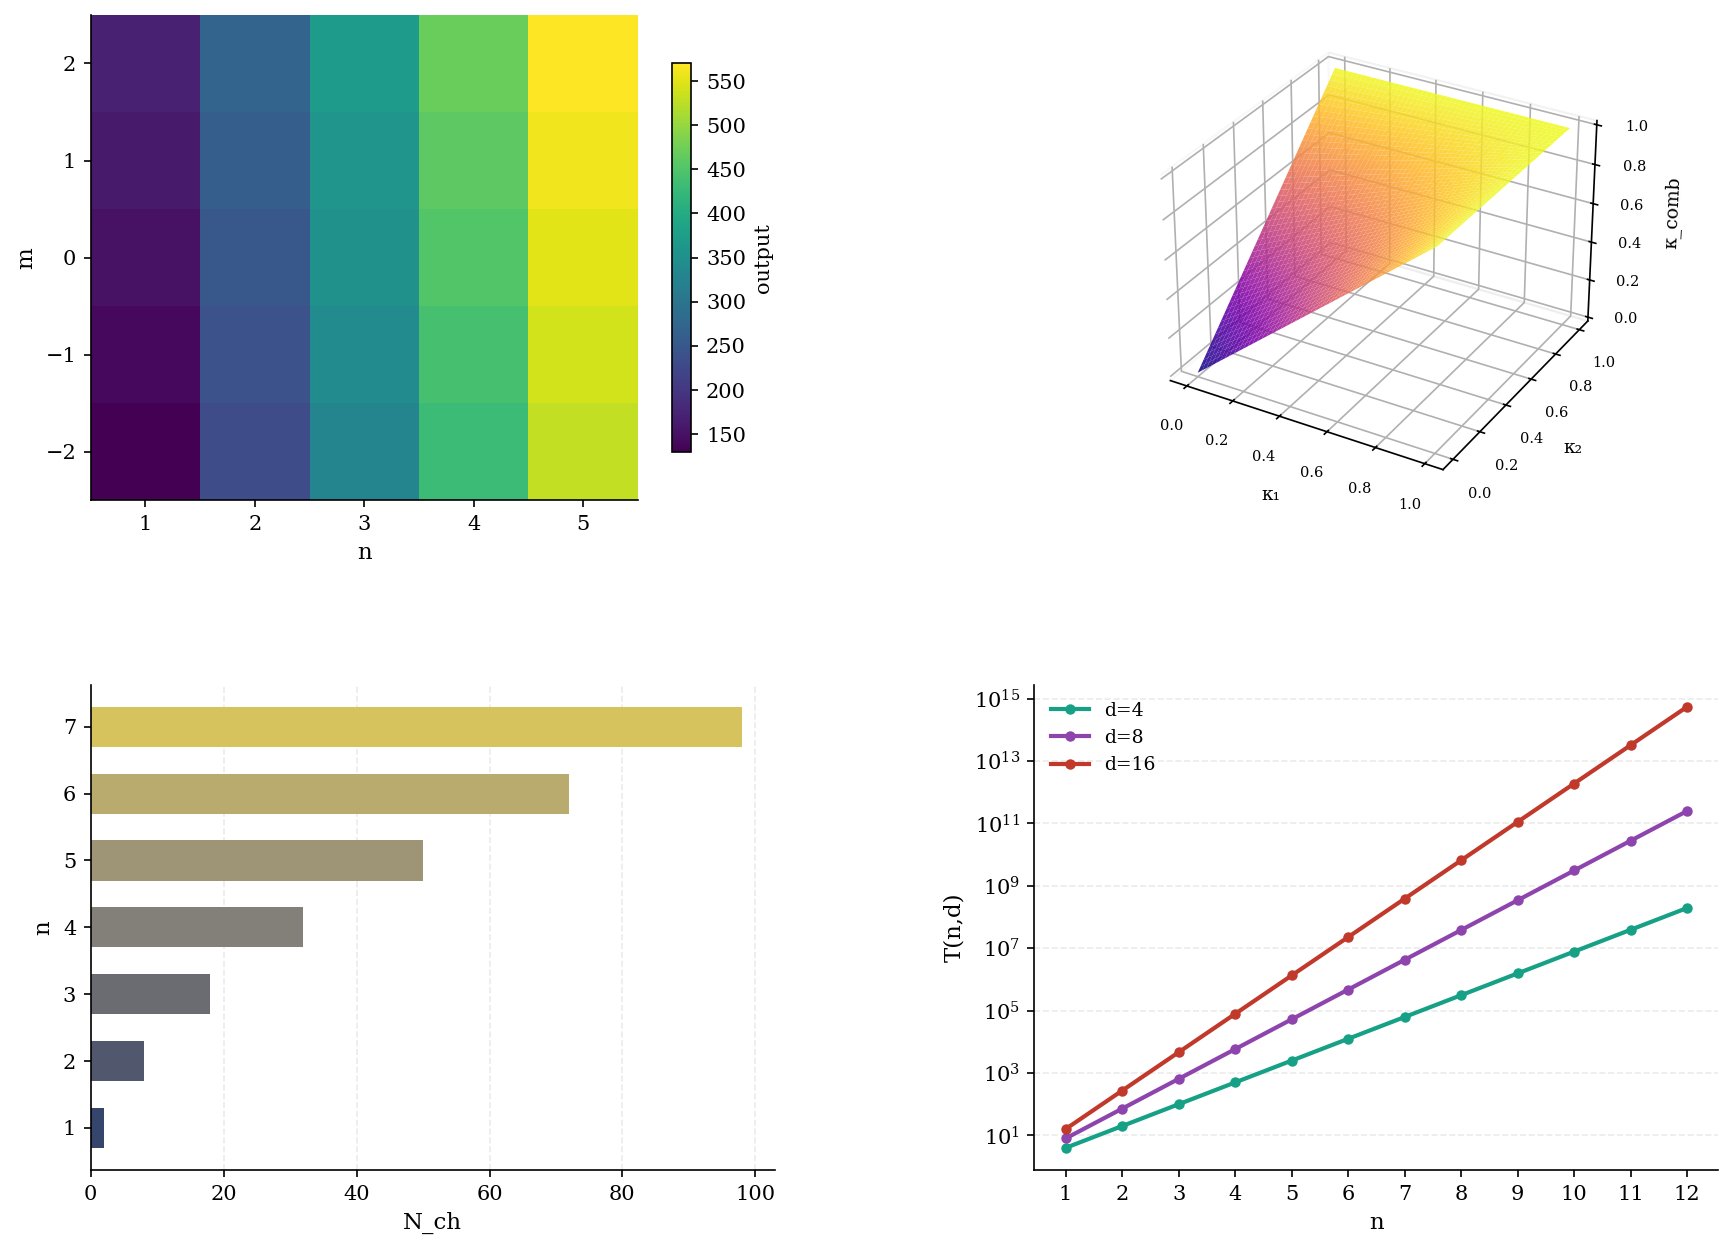
\includegraphics[width=\textwidth]{panel4_forest_dynamics.png}
  \caption{Forest dynamics and receiver-relative evaluation.
    \emph{Top-left}: Heatmap of the receiver-relative output
    $n{\cdot}100 + m{\cdot}10 + M$ (with $M=50$ fixed) across
    the $(n,m)$ grid; every cell is a distinct value, illustrating
    the Receiver-Relativity theorem.
    \emph{Top-right}: 3D surface of composite catalytic power
    $\kappa_{\mathrm{comb}}(\kappa_1,\kappa_2) = 1-(1-\kappa_1)(1-\kappa_2)$
    over $[0,1]^2$.
    \emph{Bottom-left}: Forced channel count $N_{\mathrm{ch}}=2n^2$
    per depth level (horizontal bars).
    \emph{Bottom-right}: Trajectory encoding capacity $T(n,d)$ for
    $d\in\{4,8,16\}$ and $n=1,\ldots,12$; log scale.}
  \label{fig:panel4}
\end{figure*}

% ============================================================
\section{Discussion}
\label{sec:discussion}

\subsection{Limitations}

\paragraph{No global consistency.}
\srn\ provides no global consistency guarantee.  Two nodes in different
partition regions may evaluate the same expression to values that
cannot be reconciled by any third observer.  This is by design:
receiver-relativity is a feature, not a defect.  Applications that
require global consensus must build it explicitly as a meta-expression
layer.

\paragraph{Registry divergence.}
Since registries are local and updates are propagated by forwarded
expressions, a node that is temporarily unreachable may fall behind.
There is no catch-up mechanism in the core language.  A meta-expression
could implement one.

\paragraph{Timing resolution.}
The transmission encoding (Definition~\ref{def:encoding}) requires the
substrate to provide timing resolution sufficient to distinguish adjacent
$\Delta P$ values.  On commodity hardware, nanosecond resolution is
available; on lossy links, the effective resolution may be lower.  The
number of distinguishable expressions per unit time scales as
$T(n, d) = d(1+d)^{n-1}$; lower timing resolution reduces effective
$d$.

\paragraph{No garbage collection.}
The live registry is append-biased with no eviction policy.  Long-running
nodes accumulate registry entries indefinitely.  Applications must
implement eviction as a meta-expression.

\subsection{Open Problems}

\begin{enumerate}[noitemsep,topsep=2pt]
\item \emph{Bisimulation}: Is there a natural notion of bisimulation
  for \srn\ processes analogous to CCS bisimulation~\cite{milner1989communication}?
\item \emph{Type-theoretic interpretation}: Can the partition coordinate
  system be interpreted as a dependent type system?
\item \emph{Expressiveness}: What is the computational class of \srn?
  Is it Turing-complete?
\item \emph{Convergence}: Under what conditions does repeated application
  of a catalyst cascade converge to $\floor$?
\item \emph{Forest dynamics}: Can the Forest Theorem be strengthened
  to include topological properties of the emerging network graph?
\end{enumerate}

\subsection{Comparison with Related Work}

\paragraph{Mobile ambients~\cite{cardelli2000mobile}.}
Cardelli and Gordon's ambient calculus allows processes to move between
named locations.  \srn\ also moves code (via \texttt{forward}), but
locations are partition coordinates rather than names.  The key
difference: ambient names are administrative; partition coordinates are
physically grounded.

\paragraph{Chemical abstract machine~\cite{berry1992chemical}.}
Berry and Boudol's CHAM treats reduction as a chemical reaction:
molecules float freely and react when they meet.  \srn\ is similar in
that composition (\lstinline|<>|) is context-free.  The key difference:
CHAM reactions are unordered; \srn\ evaluation is receiver-relative.

\paragraph{CPS and continuations~\cite{plotkin1975call}.}
\srn\ expressions are not continuation-passing style; they are
evaluated eagerly at the receiver.  The sequential operator \lstinline|;|
provides continuation-like chaining.

\paragraph{Pi-calculus~\cite{milner1992pi}.}
The $\pi$-calculus transmits channel names, enabling dynamic
reconfiguration.  \srn\ transmits expressions; the registry plays the
role of the channel environment.  The key difference: \srn\ has no
bound names in the transmission; partition coordinates are public.

% ============================================================
\section{Conclusion}
\label{sec:conclusion}

Sango Rine Shumba is a forest.  Not a garden.  Not a network
administered from a centre and organised around a shared protocol.
A wild ecosystem in which structure is what individuals make it, and
where the making never stops.

The four mathematical foundations---individuation by negation,
partition coordinates, the entropic floor, and cross-representation
composition freedom---are not design choices.  They are derivable from
first principles, and any language that takes them seriously arrives
at a design close to \srn.  The mandatory \lstinline|not| boundary
encodes individuation; the $(n,\ell,m,s)$ coordinate system encodes
position in partition space; the floor $\floor > 0$ explains why
receiver-relativity is not an approximation; and the \lstinline|<>|
operator encodes the apples-and-oranges freedom.

The Forest Theorem says what this produces: a network in which
membership equals capability, in which there is no authority that
precedes participation, and in which the structure is entirely the
aggregate of what the participants do.  Any machine that evaluates
\srn\ expressions is already in the forest.  No invitation is needed.

The security is structural.  Replay immunity comes from the arrow of
time.  Boundary forgery resistance comes from the inaccessibility of
another node's partition state.  Incorruptibility comes from the
absence of a parser.  These properties hold as long as the physical
substrate has an arrow of time and maintains locality of state.  They
do not depend on any computational hardness assumption.

Sango rine shumba.  The lions are the individuals.  The forest is what
they make by being what they are.

% ============================================================
\section*{Acknowledgements}

The author thanks the wild forest for not requiring acknowledgement.

% ============================================================
\bibliographystyle{plainnat}
\bibliography{references}

\end{document}
